\documentclass[12pt,spanish,oneside, a4paper]{book}
\usepackage{lmodern}
\usepackage{amssymb,amsmath}
\usepackage{ifxetex,ifluatex}
\usepackage{fixltx2e} % provides \textsubscript
\ifnum 0\ifxetex 1\fi\ifluatex 1\fi=0 % if pdftex
  \usepackage[T1]{fontenc}
  \usepackage[utf8]{inputenc}
\else % if luatex or xelatex
  \ifxetex
    \usepackage{mathspec}
  \else
    \usepackage{fontspec}
  \fi
  \defaultfontfeatures{Ligatures=TeX,Scale=MatchLowercase}
\fi
% use upquote if available, for straight quotes in verbatim environments
\IfFileExists{upquote.sty}{\usepackage{upquote}}{}
% use microtype if available
\IfFileExists{microtype.sty}{%
\usepackage{microtype}
\UseMicrotypeSet[protrusion]{basicmath} % disable protrusion for tt fonts
}{}
\usepackage[inner = 3cm, outer = 2cm, top = 2.5cm, bottom = 2.5cm]{geometry}
\usepackage{hyperref}
\hypersetup{unicode=true,
            pdfauthor={Paola Corrales},
            pdfborder={0 0 0},
            breaklinks=true}
\urlstyle{same}  % don't use monospace font for urls
\ifnum 0\ifxetex 1\fi\ifluatex 1\fi=0 % if pdftex
  \usepackage[shorthands=off,main=spanish]{babel}
\else
  \usepackage{polyglossia}
  \setmainlanguage[]{spanish}
\fi
\usepackage{longtable,booktabs}
\usepackage{graphicx,grffile}
\makeatletter
\def\maxwidth{\ifdim\Gin@nat@width>\linewidth\linewidth\else\Gin@nat@width\fi}
\def\maxheight{\ifdim\Gin@nat@height>\textheight\textheight\else\Gin@nat@height\fi}
\makeatother
% Scale images if necessary, so that they will not overflow the page
% margins by default, and it is still possible to overwrite the defaults
% using explicit options in \includegraphics[width, height, ...]{}
\setkeys{Gin}{width=\maxwidth,height=\maxheight,keepaspectratio}
\IfFileExists{parskip.sty}{%
\usepackage{parskip}
}{% else
\setlength{\parindent}{0pt}
\setlength{\parskip}{6pt plus 2pt minus 1pt}
}
\setlength{\emergencystretch}{3em}  % prevent overfull lines
\providecommand{\tightlist}{%
  \setlength{\itemsep}{0pt}\setlength{\parskip}{0pt}}
\setcounter{secnumdepth}{5}
% Redefines (sub)paragraphs to behave more like sections
\ifx\paragraph\undefined\else
\let\oldparagraph\paragraph
\renewcommand{\paragraph}[1]{\oldparagraph{#1}\mbox{}}
\fi
\ifx\subparagraph\undefined\else
\let\oldsubparagraph\subparagraph
\renewcommand{\subparagraph}[1]{\oldsubparagraph{#1}\mbox{}}
\fi

%%% Use protect on footnotes to avoid problems with footnotes in titles
\let\rmarkdownfootnote\footnote%
\def\footnote{\protect\rmarkdownfootnote}

%%% Change title format to be more compact
\usepackage{titling}

% Create subtitle command for use in maketitle
\newcommand{\subtitle}[1]{
  \posttitle{
    \begin{center}\large#1\end{center}
    }
}

\setlength{\droptitle}{-2em}
  \title{}
  \pretitle{\vspace{\droptitle}}
  \posttitle{}
\subtitle{Validación de parametrizaciones de capa límite utilizando datos de radar}
  \author{Paola Corrales}
  \preauthor{\centering\large\emph}
  \postauthor{\par}
  \date{}
  \predate{}\postdate{}

\usepackage{booktabs}
\usepackage{longtable}
\usepackage{array}
\usepackage{multirow}
\usepackage[table]{xcolor}
\usepackage{wrapfig}
\usepackage{float}
\usepackage{colortbl}
\usepackage{pdflscape}
\usepackage{tabu}
\usepackage{threeparttable}
\usepackage[normalem]{ulem}

\usepackage{setspace}
\setstretch{1.5}
\usepackage{subfig}
\usepackage{hyperref}
\usepackage[textsize=tiny]{todonotes}

\begin{document}

\begin{titlepage}
    \centering
    \includegraphics[width=0.2\textwidth]{logoUBA}  \hfill \includegraphics[width=0.2\textwidth]{logoDCAO} \par
    \vspace{1cm}
    {\scshape\LARGE Universidad de Buenos Aires  \\
    \large Facultad de Ciencias Exactas y Naturales \\
Departamento de Ciencias de la Atmósfera y los Océanos  \par}
    \vspace{0.5cm}
    {\scshape\Large Tesis de Licenciatura en Ciencias de la Atmósfera\par}
    \vspace{1.5cm}
    {\huge\bfseries Validación de parametrizaciones de capa límite utilizando datos de radar\par}
    \vspace{4.5cm}
    {\Large Tesista: Paola \textsc{Corrales} \\
        Directores: Dr. Jua \textsc{Ruíz} y Dra. Marisa \textsc{Gassmann}
    \par}
    \vfill

% Bottom of the page
    {\large --2018--\par}
\end{titlepage}

\renewcommand{\listtablename}{Índice de tablas} 
\renewcommand{\tablename}{Tabla} 

\chapter*{Agradecimientos}

A mi gata

\newpage

\chapter*{Resumen}\begin{center}\begin{minipage}{\dimexpr\paperwidth-7cm}
Este es el resumen de mi tesis sdfklsadjksajdlkf skjdfklsdflkkflsjfadfkxvxkcn  sdfjskdjskd osdfmfk sdfkjlls 
\end{minipage}
\end{center}\newpage

\setcounter{tocdepth}{4} \tableofcontents

\listoffigures
\newpage

\listoftables
\newpage

\chapter{Introducción}\label{introduccion}

La capa límite planetaria (CLP) corresponde a la porción de atmósfera
que se encuentra directamente influenciada por la superficie terrestre y
que responde a sus forzantes en una escala de tiempo de una hora o menos
(Stull, 1988). Dentro de esta capa el flujo se encuentra en estado
turbulento y por lo tanto los movimientos del aire son aleatorios.
Debido a que la capa límite es forzada por las características de la
superfice terrestre (por su rugosidad, temperatura, humedad y otros) su
evolución sigue un ciclo con variabilidad diaria.

La estructura de la capa límite puede ser descripta a partir de su
evolución. Luego del amanecer la capa límite comienza a crecer debido al
calentamiento radiativo de la superficie que produce turbulencia dando
lugar a la capa mezclada. En esta capa la intensidad del viento, la
temperatura potencial y otras variables se mantienen constantes con la
altura debido a la intensa mezcla vertical, persistiendo a lo largo del
día hasta el momento del atardecer cuando la turbulencia comienza a
decaer. Durante la noche se forma la capa límite nocturna estable
forzada por el enfriamiento radiativo desde superficie, caracterizada
generalmente por una inversión en el perfil de temperatura. En esta capa
la turbulencia puede decaer o producirse intermitentemente. Por encima
de esta capa persisten las características de la capa mezclada por lo
que toma el nombre de capa residual y no forma parte de la capa límite.
Al amanecer se forma una nueva capa mezclada que orada la capa estable
hasta hacerla desaparecer.

Los procesos que ocurren dentro de esta capa son de suma importancia
para entender y pronosticar la evolución de la tropoósfera en distintas
escalas espaciales y temporales. En particular estos procesos controlan
el intercambio de energía entre la superficie y la atmósfera afectando,
entre otras cosas, las condiciones para la ocurrencia de convección
húmeda profunda y la intensidad de las circulaciones de mesoescala,
originando eventos meteorológicos que pueden tener un alto impacto sobre
las actividades humanas.

En nuestra región existen estudios que buscan caracterizar la evolución
y los procesos que ocurren en la capa límite de forma tal de poder
avanzar en su entendimiento y su dependencia por ejemplo con las
propiedades de la superficie o el estado de la atmósfera (Mazzeo y
Gassmann, 1990; Ulke, 2000; Gassmann y Mazzea, 2001; Acevedo et~al.,
2014; Tonti y Gassmann, 2015).

Dado que la ocurrencia de turbulencia en la capa límite planetaria se da
en múltiples escalas espaciales y temporales, la representación de los
procesos que ocurren dentro de ella es un desafío para los modelos
numéricos. Actualmente los modelos de simulación regional y global no
cuentan con la resolución necesaria para representar los procesos de la
CLP de forma explícita, debiendo recurrir a una representación
simplificada. De esta manera se simula numéricamente una parte del
espectro turbulento, mientras que los procesos en la escala de subgrilla
se resuelven a través de parametrizaciones con cierres de distinto orden
(Stull, 1988), es decir, con diferentes niveles de aproximaciones.

Existen diferentes alternativas para parametrizar los procesos de capa
límite pero pueden clasificarse en dos grandes grupos. De acuerdo a
Stull (1988), las parametrizaciones con clausura local determinan el
valor de cualquier variable desconocida en cada punto a partir del valor
o el gradiente de una variable conocida en el mismo punto; suponiendo
que la difusión turbulenta tiene un comportamiento análogo al de la
difusión molecular. Por otro lado, las parametrizaciones con clausura no
local asumen que la turbulencia está caracterizada por la superposición
de torbellinos de distintas escalas que transportan las características
del medio; y para lograr esto, el valor de la variable desconocida en un
punto es aproximada a partir de una variable conocida en varios puntos
en el espacio.

La validación de las diferentes parametrizaciones de CLP en distintas
situaciones sinópticas es un tema de gran interés debido a la necesidad
de modelar los procesos de subgrilla presentes que afectan procesos en
el resto de las escalas de variabilidad atmosférica (Zhang y Zheng,
2004; Hu et~al., 2010; Xie et~al., 2012; Banks et~al., 2016).

A nivel regional, la representación de la capa límite en los modelos
numéricos ha recibido mucha atención en las zonas oceánicas
(particularmente en los océanos tropicales, Wang et~al. (2004)). Sin
embargo, existen pocos estudios acerca del desempeño de las
parametrizaciones de capa límite en las regiones continentales (Ulke y
Andrade, 2001; Ruiz et~al., 2010; Berri et~al., 2012; Rizza et~al.,
2013).

Uno de los principales desafíos a la hora de estudiar los procesos que
ocurren en la capa límite o para validar cómo los modelos representan
dichos procesos, es la disponibilidad de observaciones. Las redes de
radiosondeos que permiten obtener perfiles de viento, temperatura y
humedad en la capa límite miden con frecuencias temporales de entre 12 y
24 horas (sólo eventualmente cada 6 horas) lo que dificulta la
posibilidad de analizar la evolución de las características de la CLP a
lo largo del día. Sumado a esto, las mediciones se realizan en puntos
geográficos individuables y muy dispersos entre sí.

Sin embargo los radares Doppler permiten estimar la componente radial
del viento en un radio horizontal de hasta 240 km y a partir de esa
información reconstruir perfiles verticales de viento utilizando la
técnica Velocity Azimuth Display (VAD). Otra ventaja de las
observaciones de radar es que están disponibles con una frecuencia
temporal de hasta 5 minutos permitiendo obtener perfiles de viento con
una resolución temporal mucho mayor que la de los radiosondeos.

En días en los que no existen ecos producidos por hidrometeoros, los
radares pueden detectar el viento dentro de la capa límite a partir de
blancos como los insectos. De acuerdo a Rennie et~al. (2010) estos datos
podrían ser utilizados si se elimina el efecto de los ecos de terreno y
otras observaciones erróneas.

La calidad de estos perfiles ha sido comparada con los perfiles
obtenidos a partir de radiosondeos, encontrándose en general que los
datos obtenidos resultan adecuados para su uso en el estudio de los
procesos de capa límite y en la verificación de modelos numéricos
(Bousquet et~al., 2008; Salonen et~al., 2008) y en la generación de
condiciones iniciales para pronósticos a muy corto plazo (Rennie et~al.,
2011).

Uno de los aspectos importantes a tener en cuenta en el uso de radares
para el estudio de los perfiles de viento, es la necesidad de aplicar un
riguroso control de calidad a los datos que permita solucionar diversos
aspectos que pueden afectar la confiabilidad de los mismos. Entre los
problemas más comunes se cuentan: contaminación por ecos de terreno,
efecto de aliasing, y contaminación por blancos móviles. Estos aspectos
deben ser abordados antes de poder utilizar los datos para estimar el
perfil de velocidad del aire (Holleman et~al., 2008; Rennie et~al.,
2011) aplicando algoritmos de control de calidad (Rennie et~al., 2011;
Ruiz et~al., 2015).

La disponibilidad de la información de radar Doppler en Argentina
comienza en 1999 con la instalación del radar Ezeiza (Elía et~al.,
2017), ofreciendo un gran recurso de información para estudiar las
propiedades de la capa límite planetaria en nuestra región y para
validar la calidad de los modelos numéricos a la hora de representar
dichas propiedades.

El objetivo de esta Tesis de Licenciatura es desarrollar una metodología
para el estudio de los procesos de capa límite a partir de los datos de
radar Doppler y analizar el comportamiento de tres parametrizaciones de
CLP disponibles en el modelo Weather Research and Forecasting (WRF -
Skamarock et~al. (2008)) al representar algunos de los procesos
presentes en uno de los casos de estudio seleccionados.

Se plantea como hipótesis que los datos de viento radial obtenidos de
información de radar permiten realizar buenas estimaciones de los
perfiles verticales de viento con una frecuencia temporal de hasta 5
minutos, en un espesor que abarca desde los 100 metros desde la
superficie y hasta 2000 o 3000 m de altura dependiendo de la altura de
la capa límite, la presencia de nubes y otras condiciones. La alta
frecuencia de información observacional ofrece la posibilidad de
caracterizar la evolución temporal de dichos perfiles dentro de la capa
límite atmosférica. La estimación de esos perfiles permitirán además
validar las parametrizaciones de la capa límite que utilizan los modelos
numéricos con una mayor resolución temporal y espacial a la utilizada en
trabajos previos.

\chapter{Metodología}\label{metodologia}

En esta sección se describen los datos utilizados en el trabajo, la
metodología desarrollada para alcanzar el objetivo propuesto. En primer
lugar se determinaron las características necesarias para identificar
posibles casos de estudio que permitan analizar los procesos de CLP
asociados al ciclo diario. Luego se procesó los datos de radar para caso
en estudio y se aplicaron los controles de calidad necesarios antes de
realizar el cálculo del VAD desarrollado y validado como parte de este
trabajo. Se analizó la consistencia de los resultados obtenidos y las
características principales de la variación del viento a lo largo del
día haciendo especial hincapié en los procesos que ocurren en el período
nocturno. Para las simulaciones numéricas con el modelo regional WRF se
definió un dominio y las condiciones iniciales adecuadas para modelar un
caso de estudio utilizando tres parametrizaciones disponibles en el
modelo. Se compararon las simulaciones con las observaciones previamente
obtenidas y se analizaron algunas variables asociadas a la turbulencia.

\section{Región y casos de estudio}\label{region-y-casos-de-estudio}

Este trabajo centra el análisis en la región de la ciudad de Paraná
(provincia de Entre Ríos, Argentina) donde se encuentran el Radar
Doppler del INTA (Instituto Nacional de Tecnología Agropecuaria) y una
estación meteorológica de superficie perteneciente al SMN (Servicio
Meteorológico Nacional) separados por aproximadamente 9 kilómetros de
distancia.

\begin{figure}

{\centering \includegraphics{Tesis_files/figure-latex/topografia-1} 

}

\caption[Topografía de la región en estudio en metros sobre el nivel del mar.]{Topografía de la región en estudio en metros sobre el nivel del mar. El punto negro indica la ubicación del Radar INTA Paraná, el punto rojo indica la ubicación de la estación Paraná Aero. Datos ETOPO1 1 Arc-Minute Global Relief Model NOAA (Amante y Eakins, 2009). \label{topografia}}\label{fig:topografia}
\end{figure}

La elevación de la región elegida muestra un mínimo de 5 metros sobre el
nivel del mar en el lecho del río Paraná y un máximo de aproximadamente
110 metros sobre el nivel del mar sobre el margen sudeste de río donde
ubica tanto la estación meteorológica como el radar (Figura
\ref{topografia}). La región está dominada por la presencia del río y
las regiones costeras donde predominan los campos de pastizales o pasto
con excepción la ciudad de Paraná (al norte), la ciudad de Santa Fé (al
noreste) y pequeños conglomerados de casas.

\subsection{\texorpdfstring{Criterios utilizados para la selección de
los casos de estudio
\label{sec-criterios}}{Criterios utilizados para la selección de los casos de estudio }}\label{criterios-utilizados-para-la-seleccion-de-los-casos-de-estudio}

Se determinaron distintos criterios para poder identificar casos de
estudio donde se observe el desarrollo de la CLP en condiciones normales
\textbf{Cita}.

Al mismo tiempo se buscaron situaciones donde los datos de radar son
confiables. Los criterios seleccionados son los siguientes:

\begin{itemize}
\tightlist
\item
  \textbf{Viento moderado.} En estas situaciones los datos de radar son
  más confiables y permiten el desarrollo de la capa límite estable
  nocturna (Gassmann y Mazzea, 2001). Se determinó como umbral máximo 7
  m/s que corresponde a la categoría de brisa moderada en la escala de
  Beaufort.
\item
  \textbf{Cielos despejados.} Para garantizar el calentamiento desde la
  superficie y el desarrollo de una capa límite mezclada. En los casos
  donde hubo nubosidad presente, se analizó el tipo de nubosidad, el
  porcentaje de cobertura del cielo y el impacto que tuvo en la
  temperatura. Los días donde la nubosidad afectó la variación normal de
  la temperatura (descenso continuo por la noche y ascenso durante el
  día) fueron descartados.
\item
  \textbf{Verano.} Donde el calentamiento es más intenso.
\end{itemize}

Las características previas se buscaron a partir del análisis de los
datos de la estación meteorológica de superficie Paraná Aero provistos
por el SMN y de reflectividad (dBZ) del radar de Paraná para el mes de
enero de 2016.

En el primer tipo de datos se analizó la velocidad de viento, la
cobertura nubosa y la precipitación observada a cada hora. En el caso de
los datos de radar se observó la presencia de ecos meteorológicos en las
inmediaciones del radar (a una distancia menor a 150 km) en cada tiempo
disponible (aproximadamente cada 10 minutos). Un caso de estudio posible
será aquel que cumpla con las características mencionadas durante las 24
horas del día aunque es deseable que las condiciones se mantengan
durante las 12 horas previas al día en estudio ya que las
características de la capa estable nocturna puede ser influenciada por
las características de la capa mezclada del día anterior.

\section{Descripción de los datos de
radar}\label{descripcion-de-los-datos-de-radar}

El radar ubicado en Paraná (Provincia de Entre Ríos) es de doble
polarización y emite energía electromagnética en la banda C (4 a 8 GHz).
La estrategia de escaneo de la atmósfera está programada para que la
antena dé giros en sentido horizontal de 360º y cambie de elevación
sucesivamente 12 veces. El ángulo vertical varía entre 0.5° y 15.1°. El
rango del radar (distancia a la que llega la señal desde la ubicación
del radar) puede ser de 120, 240 y 480 km con una resolución espacial en
la dirección del rango de 500 m de acuerdo a la estrategia de escaneo
(Saibene et~al., 2014).

El escaneo completo del volumen de atmósfera que rodea al radar se
realiza cada 5 minutos en el rango de 120 km y de 240 km de manera
intercalada, dando como resultado 144 volúmenes de datos diarios para
cada estrategia de escaneo. Las variables disponibles en cada tiempo
incluyen la reflectividad (dBZ) y velocidad radial (\(V_r\)).

Los datos de reflectividad permitieron evaluar la presencia de nubosidad
en cada momento mientras que la velocidad radial se utilizó para
calcular el perfil de viento. La velocidad radial medida por el radar
corresponde a la velocidad de un objetivo u obstáculo en el camino del
haz. En situaciones de aire claro (sin nubosidad) es posible tener una
medida del campo de viento dentro de la capa límite usando insectos como
obstáculos.

En este trabajo se usaron datos de radar provistos por el Servicio
Meteorológico Nacional correspondientes a la estrategia de 240 km y 12
ángulos de elevación para los periodos comprendidos por cada caso de
estudio. Los datos correspondientes a la estrategia de 120 km no fueron
utilizados debido a la cantidad de ángulo de elevación disponibles fue
distinta para cada día y en todos los casos menor a 12.

Cada volumen de dato correspondiente a un tiempo de escaneo completo fue
convertido al formato CfRadial con el paquete Radx C++ (Dixon, 2010 NCAR
- National Center for Atmospheric Research) para el posterior
procesamiento y análisis. En particular se utilizó la variable de
reflectividad sin procesamiento para determinar la presencia o no de
ecos meteorológicos en el dominio cercano al radar y la velocidad radial
para la obtención de los perfiles de viento.

\section{Tratamiento de aliasing}\label{tratamiento-de-aliasing}

Un problema importante al momento de utilizar los datos de velocidad
radial es la contaminación por aliasing ya que afecta significativamente
la calidad de los perfiles de viento finales, de acuerdo a Gao y
Droegemeier (2004) un 3\% de contaminación por aliasing puede generar un
error cuadrático medio del 50\% en el perfil de viento medio a partir de
la técnica VAD. El aliasing es la superposición de la señal de radar y
ocurre cuando la velocidad real supera a la velocidad de Nyquist
(\(V_N\)). Este parámetro es intrínseco a las características del radar
ya que depende de la frecuencia y estrategia de escaneo y en particular
de la frecuencia de repetición del pulso o señal que emite.

En el caso del radar de Paraná con la estrategia de escaneo de 240km de
rango, tiene una \(V_N = 6.7 m/s\) por lo que cualquier velocidad mayor
se verá afectada por el aliasing. Esto puede verse en la Figura
\ref{aliasing}, las regiones con aliasing son aquellas que donde el
valor de la velocidad radial salta al extremo opuesto de la escala.

Existen muchos algoritmos que buscan solucionar el problema del aliasing
(por ejemplo Haase y Landelius, 2004; Lim y Sun, 2010) con distinto
grado de éxito. Una opción válida es el algoritmo de corrección de
aliasing basado en regiones similares disponible en la librería PyART
(Helmus y Collis, 2016) disponible en Collis (2016). Este algoritmo
busca regiones con velocidad radial similar y transforma el rango de la
variable hasta que todas las regiones fueron corregidas de tal manera de
obtener un campo continuo. El campo de velocidad radial sin aliasing
obtenido utilizando este algoritmo se muestra en la Figura
\ref{no-aliasing}.

A partir de la exploración visual puede observarse que el algoritmo
resuelve el problema de manera satisfactoria en mayor parte del dominio.
Sin embargo se observa una zona en el borde inferior donde la magnitud
de la variable es anómalamente alta. Algunas discontinuidades se
observaron también en otros casos. Se decidió utilizar este algoritmo
para preprocesar todos los volúmenes de datos de radar y se incorporaron
algunos controles de calidad al algoritmo de VAD desarrollado (Ver
Sección \ref{sec-vad}).

\begin{figure}

{\centering \subfloat[Con aliasing \label{aliasing}\label{fig:aliasing1}]{\includegraphics[ ]{Tesis_files/figure-latex/aliasing-1} }\subfloat[Sin aliasing \label{no-aliasing}\label{fig:aliasing2}]{\includegraphics[ ]{Tesis_files/figure-latex/aliasing-2} }

}

\caption{Velocidad radial (m/s) observada a las 06 UTC por el radar de Paraná en la elevación $1.3^{\circ}$ y $V_N = 6.7 m/s$. Notar las escalas diferentes.}\label{fig:aliasing}
\end{figure}

\section{\texorpdfstring{Visualización Azimutal de la Velocidad
\label{sec-vad}}{Visualización Azimutal de la Velocidad }}\label{visualizacion-azimutal-de-la-velocidad}

A medida que el radar rota en la dirección azimutal, mide la velocidad
de los objetivos para cada ángulo y rango de manera continua y en
función del azimut. A esto se le da el nombre de Visualización Azimutal
de la Velocidad o por sus siglas en inglés VAD (por Velocity Azimuth
Display, Lhermitte (1962)) y se muestra en la Figura \ref{vad}. Si el
campo de viento es horizontalmente homogéneo, la velocidad radial media
tiene un comportamiento sinusoidal en función del azimut.

\begin{figure}

{\centering \includegraphics{Tesis_files/figure-latex/vad-1} 

}

\caption{Velocidad radial (m/s) en función del azimut (grados) para un rango y ańgulo de elevación fijos. En color se  ajusta una función sinusoidal a los datos. \label{vad}}\label{fig:vad}
\end{figure}

Esta variable corresponde es la componente radial del viento, es decir,
la proyección del viento en la dirección de la propagación del haz de
radar. Los valores negativos corresponden a movimiento hacia el radar y
valores positivos movimientos desde el radar, mientras que el valor nulo
ocurre en las regiones donde el viento es perpendicular a la trayectoria
del haz y por lo tanto su proyección es cero.

En días de buen tiempo y aire claro la señal que recibe el radar
corresponden a los insectos que se encuentran en la capa límite.
Diferentes autores han analizado la validez de la estimación del viento
a partir de estos blancos. Si bien en algunos casos los insectos pueden
ser considerados blancos pasivos, en otros casos, dependiendo del tamaño
y características del insecto, pueden moverse con velocidad y dirección
propias (Rennie, 2014). De acuerdo a Hannesen et~al. (2014), una posible
solución a este problema podría ser el uso de variables polarimétricas
que permitan determinar la orientación y dirección de desplazamiento de
los insectos para luego corregir la variable \(V_r\) observada. En este
trabajo si bien no se analizó la calidad de los datos desde este punto
de vista individualmente, si se tuvieron en cuenta controles de calidad
para disminuir errores.

Usando el concepto de la Visualización Azimutal de la Velocidad
distintos autores han desarrollado técnicas para obtener el perfil
vertical de viento real a partir del viento radial o su gradiente con
diferentes grados de complejidad. Estas técnicas son también son
llamadas VAD (o sus derivaciones). Algunos de estos algoritmos permiten
estimar variaciones del viento dentro del dominio siempre que éstas sean
lineales. Browning y Wexler (1968), unos de los primeros autores en
aplicar este concepto, desarrolló una técnica utilizando series de
Fourier para obtener variables del campo del viento descompuesto en la
parte divergente, la parte rotacional y la componente de deformación
válida para casos donde el campo de viento es horizontalmente homogéneo.

Una variación del VAD, el EVAD (por las siglas en inglés de
Visualización Azimutal de la Velocidad Extendida) fue desarollado por
Matejka y Srivastava (1991). En esta técnica se incorpora el uso de
pesos al estimar las variables para tener en cuenta los errores en los
datos originales y el análisis de los residuos obtenidos a partir de las
regresiones calculadas. De acuerdo a los autores, esto permite el uso
del algoritmo en situaciones donde la cortante vertical del viento es
fuerte, inhomogeneidades en el campo horizontal o insuficientes datos de
radar. Posteriormente Gao et~al. (2004) desarrolló el GVAD (por las
siglas en inglés de Visualización Azimutal del Gradiente de la
Velocidad) que permite obtener el perfil vertical del viento aún en
casos donde los datos están contaminados por aliasing utilizando el
gradiente del la velocidad radial. Si bien esta técnica es una mejora
sustancial, es muy sensible a errores aleatorios y sistemáticos causados
por el aliasing. Xu et~al. (2010) también busca solucionar el problema
de la contaminación por aliasing utilizando un algoritmo que ajusta los
datos con aliasing a un modelo de viento uniforme. Posteriormente el
mismo autor modifica este algoritmo a partir de un un método variacional
que permite eliminar la condición de homogeneidad del campo de viento.

Para esta tesis se desarrolló un algoritmo para el cálculo del VAD
siguiendo a Browning y Wexler (1968) debido a la simpleza de la técnica
pero además se incluyeron controles de calidad específicos para asegurar
la validez de los resultados, algunos de los cuales también fueron
implementados por los autores mencionados.

\subsection{Desarrollo matemático}\label{desarrollo-matematico}

El viento radial medido por el radar para un ángulo de elevación
\(\theta\) y rango \(r\) determinado puede expresarse en función del
azimut \(\phi\):

\begin{equation}
\label{eq-vr1}
V_r =  v \cos(\theta) \cos(\phi) + u \cos(\theta) \sin(\phi) - w \sin(\theta)
\end{equation}

Donde \(u\), \(v\) y \(w\) son las componentes del viento en coordenadas
cartesianas.

La Ecuación \ref{eq-vr1} puede ser expresada como suma de una serie de
Fourier de la forma:

\begin{equation}
\label{eq-vr2}
V_r =  \frac{1}{2}a_0 + \sum_{n = 1}^{\infty} (a_n \cos(n\phi) + b_n \sin(n \phi)) 
\end{equation}

Para \(n=1\), los coeficientes de Fourier están asociados al viento en
el centro del dominio de escaneo (con subíndice 0) como:

\begin{equation} \label{eq-vr3}
\begin{aligned}
a_0 = r \cos(\theta)\left ( \frac{\overline{\partial u}}{\partial x} + \frac{\overline{\partial v}}{\partial y} \right) + 2 w \sin(\theta) \\
a_1 = u_0 \cos(\theta) \\
b_1 = v_0 \cos(\theta) \\
a_2 = \frac{1}{2} r \cos(\theta)\left ( \frac{\overline{\partial u}}{\partial x} - \frac{\overline{\partial v}}{\partial y} \right) \\
b_2 = \frac{1}{2} r \cos(\theta)\left ( \frac{\overline{\partial u}}{\partial y} + \frac{\overline{\partial v}}{\partial x} \right)
\end{aligned}
\end{equation}

A partir de esto es posible ajustar cada anillo de datos de radar, es
decir los datos para cada \(\theta\) y \(r\) realizando una regresión
lineal de la forma:

\begin{equation}
\label{eq-vr4}
V_r \sim a_1\cos \phi + b_1 \sin \phi
\end{equation}

Los coeficientes \(a_0\), \(a_2\) y \(b_2\) dan información sobre la
divergencia horizontal y otras características de la variación viento.
Estos no fueron estimados por el algoritmo pero es posible su
implementación en futuros trabajos.

Finalmente la velocidad y dirección del viento pueden ser calculadas a
partir de los coeficientes (Ecuaciones \ref{eq-vr3}).

Velocidad:

\begin{equation}
\label{eq-vr5}
V = \frac{(a_{1}^{2} + b_{1}^{2})^{1/2}}{\cos(\theta)}
\end{equation}

Dirección:

\begin{equation}\label{eq-vr6}
\alpha = \frac{\pi}{2}-\tan^{-1}(\frac{a_1}{b_1}) \; \; si \; b_1 < 0 
\end{equation}\begin{equation}\label{eq-vr7}
\alpha = \frac{3\pi}{2}-\tan^{-1}(\frac{a_1}{b_1}) \; \; si \; b_1 > 0
\end{equation}

El resultado de lo anterior da un valor de la magnitud del viento y su
dirección para cada anillo asociado a un ángulo de elevación y rango
determinado. Para calcular la altura de cada anillo es necesario conocer
la propagación del haz del radar. Ésta depende del índice de refracción
de la atmósfera (N) y este a su vez de la densidad del aire y por lo
tanto de las condiciones de temperatura y humedad del momento. Existen
distintas metodologías para calcular la propagación del haz del radar
(Zeng et~al., 2014) que varían en complejidad y precisión.

En el algoritmo de VAD desarrollado se aplica el modelo 4/3 del radio de
la Tierra. Este modelo es utilizado por la mayoría de los programas de
procesamiento de datos de radar ya que pese a su simpleza (no toma en
cuenta las condiciones de la atmósfera) es aceptable para cualquier
ángulo de elevación usado, alturas máximas de entre 10 y 20 km siempre
que el gradiente de N esté alrededor de \(-1/a\) donde \(a\) es el radio
de la Tierra (Doviak y Zrnić, 1993).

Por otro lado se calcula la raíz del error cuadrático medio asociado a
cada anillo (\(rmse_a\)) para estimar la diferencia entre las
observaciones y el modelo estimado:

\begin{equation}\label{eq-vr8}
rmse_a = \sqrt {\sum \frac {(V_r - V_{rmod} )^2} {n-3}}
\end{equation}

donde \(n\) es el número de observaciones presentes en un anillo
particular.

\begin{figure}

{\centering \includegraphics{Tesis_files/figure-latex/evad-1} 

}

\caption{Velocidad del viento (m/s) en función de la altura para los distintos ángulos de elevación (puntos) y perfil final obtenido luego del primedio pesado (linea) calculados con VAD. \label{perfil-rmse}}\label{fig:evad}
\end{figure}

En la Figura \ref{perfil-rmse} se muestra el valor de la magnitud del
viento calculado a partir de cad anillo válido y en color el valor de
\(rmse_a\) asociado para un caso de ejemplo. La dispersión de los datos
varía con la altura pero se mantiene la forma del perfil con un
\(rmse_a\) medio de 2.01 m/s.

Para obtener el perfil vertical de viento que se observa en la Figura
\ref{perfil-rmse} se calcula un promedio pesado de los datos de anillos
individuales correspondientes a cada capa de atmósfera para obtener un
valor para cada punto de una grilla vertical equiespaciada
preestablecida.

El algoritmo identifica los datos de \(V\) para cualquier rango y ángulo
de elevación que se encuentran en \(z \pm d/2\) donde \(z\) es el punto
de grilla y \(d\) es la resolución espacial de la grilla vertical. Para
obtener el valor promedio de \(V\) correspondiente a la altura \(z\)
calcula un promedio pesando la variable por el \(rmse_a\) y la distancia
de cada anillo al radar \(r\). De esta manera los anillos con mayor
error y más alejados a punto donde se está estimando la velocidad y
dirección del viento tienen menor influencia en el resultado final. Si
bien el \(rmse_a\) y \(r\) tienen magnitud distinta se observó que el
primero tiene mayor influencia en el promedio pesado y que el \(r\)
permite una mayor coherencia de los datos.

\begin{equation}\label{eq-vr9}
\bar{V} = \frac {\sum w_i V_i} {\sum w_i}
\end{equation}

Donde \(w_i = \frac {1}{rmse_{ai} + r_i}\) y el subíndice \(i\) cuenta
la cantidad de datos para cada intervalo \(z \pm d/2\). De manera
análoga se calcula las componentes \(u\) y \(v\) y a partir de estas, la
dirección del viento para cada punto de grilla vertical. Este cálculo no
se realiza con la dirección del viento estimada con las Ecuaciones
\ref{eq-vr6} y \ref{eq-vr7} porque al ser una variable cíclica, el
promedio puede generar errores.

Finalmente se calcula el error de estimación asociado a cada punto de
dos maneras:

\begin{itemize}
\tightlist
\item
  \textbf{\(rmse_1\)}
\end{itemize}

\begin{equation}\label{eq-vr10} 
rmse_1 = \frac{\sigma}{\sqrt{n}}
\end{equation}

Donde \(n\) es la cantidad de anillos en esa capa y
\(\sigma^{2}= \frac{\sum (V_i - \bar{V})^2 /rmse_{ai}^2}{\sum 1/rmse_{ai}^2}\)
con \(\bar{V}\) el promedio pesado de la velocidad del viento para la
capa.

Este error relativo da cuenta de la distancia entre la velocidad
promedio calculada para ese nivel y el valor de cada anillo pesada por
el error del anillo. De esta manera si el \(rmse_{ai}\) es grande la
diferencia \((V_i - \bar{V})^2\) tiene menor peso en el error del nivel.
Es importante notar que \(V_i\) y \(\bar{V}\) no están necesariamente a
la misma altura ya que \(\bar{V}\) es el promedio de muchos \(V_i\)
dentro de una capa.

\begin{itemize}
\tightlist
\item
  \textbf{\(rmse_2\)}
\end{itemize}

\begin{equation}\label{eq-vr11}
rmse_2 = \sqrt{\frac{1}{\sum \frac{1}{rmse_{ai}^2}}}
\end{equation}

Este rmse no toma en cuenta la posible dispersión de los valores
individuales de los anillos respecto del valor medio pero retiene el
error cuadrático medio de cada anillo y calcula la raíz del error
cuadrático medio del nivel como la suma de la inversa de los errores
individuales.

\subsection{Controles de calidad de los
datos}\label{controles-de-calidad-de-los-datos}

El algoritmo de VAD desarrollado incluye algunos controles de calidad
para evitar errores asociados a problemas intrínsecos a los datos de
radar.

\subsubsection{Antes del ajuste de los
datos}\label{antes-del-ajuste-de-los-datos}

Permiten determinar cuales son los anillos de datos válidos y eliminar
posibles errores aleatorios.

\begin{itemize}
\tightlist
\item
  \textbf{Ángulos de elevación seleccionados:} La presencia de ecos de
  terreno pueden generar que los campos de velocidad radial para los
  primeros ángulos de elevación sean muy ruidosos y sin coherencia
  espacial. En el otro extremo, en caso de ser necesario,se puede
  eliminar los ángulos superiores. Por lo tanto es posible seleccionar
  el rango de ángulos a ser analizados y utilizados en el cálculo del
  VAD con el \emph{Ángulo mínimo} y el \emph{Ángulo máximo}.
\item
  \textbf{Selección del dominio de cálculo:} Otro posibilidad para
  evitar los ecos de terreno es definir un \emph{Radio interior} por
  debajo del cual no se incluyen los datos para el cálculo de VAD. En el
  otro extremo, es posible definir un \emph{Radio exterior} para limitar
  el uso de datos muy lejanos al centro del volumen de escaneo. Esto es
  importante para evitar inhomogeneidades en el campo de viento
  horizontal.
\item
  \textbf{Cantidad de datos por anillo:} el algoritmo cuenta la cantidad
  de datos válidos por anillo y se define un porcentaje de datos
  faltantes (NaN) límite respecto del total para descartar el anillo,
  por ejemplo 20\%. Si se excede al máximo definido o \emph{NaN máximo}
  el anillo es descartado. De esta manera se evita la utilización de
  anillos donde la señal es muy débil.
\item
  \textbf{Hueco continuo en un anillo:} Además de los datos faltantes
  ubicados de manera aleatoria a lo largo de un anillo, los huecos
  continuos pueden ocurrir debido a la falta de señal en una determinada
  región. De acuerdo a Matejka y Srivastava (1991) esto puede generar
  importantes errores en el resultado final, por lo tanto cuando el
  hueco o \emph{Gap máximo} es mayor a 30° de azimut, el anillo se
  descarta.
\item
  \textbf{Errores aleatorios:} Los errores aleatorios producto de ruido
  del instrumento pueden ser eliminados utilizando un filtro pasa bajo
  (Gao y Droegemeier, 2004). Este control no elimina anillos pero
  produce un suavizado de los datos de cada anillo de manera
  independiente. Es necesario definir la cantidad de datos o \(Pesos\)
  que se utilizaran para calcular el filtro en cada punto.
\end{itemize}

\subsubsection{Luego del ajuste de los
datos}\label{luego-del-ajuste-de-los-datos}

\begin{itemize}
\tightlist
\item
  \textbf{R cuadrado:} El \(r^2\) del modelo ajustado (Ecuación
  \ref{eq-vr4}) permite obtener una medida de de la calidad de ese
  modelo respecto de las observaciones. A partir de la exploración de
  resultados preliminares se observó que la definición de un umbral
  mínimo para el \(r^2\) permite descartar anillos que pese a no tener
  datos faltantes eran erróneos.
\end{itemize}

\subsection{Validación del algoritmo}\label{validacion-del-algoritmo}

Una manera posible de validar los resultados del VAD es comparando
cualitativa o cuantitativamente el perfil vertical de viento generado
con los datos de un radiosondeo en el mismo momento. Debido a la
inexistencia de sondeos en la región de Paraná se exploró la posibilidad
de utilizar datos del Radar INTA Anguil que se encuentra en la provincia
de La Pampa y radiosondeos de la estación del SMN Santa Rosa Aero. Si
bien el radar y la estación meteorológica no están en la misma
ubicación, se encuentran a unos 30 km de distancia y por lo tanto la
estación está dentro del dominio de escaneo del radar (Figura
\ref{topo-anguil}). Sin embargo se encontró que la señal de \(V_r\) en
días de cielo claro es muy pobre y por lo tanto al realizar los
controles de calidad impuestos en el algoritmo, el perfil de viento
final no llega a los 1000 m.

\begin{figure}

{\centering \includegraphics{Tesis_files/figure-latex/topo-anguil-1} 

}

\caption{Topografía de la región del radar Anguil en metros sobre el nivel del mar. El punto negro indica la ubicación del Radar INTA Anguil, el punto rojo indica la ubicación de la estación Santa Rosa Aero. Datos ETOPO1 1 Arc-Minute Global Relief Model NOAA (Amante y Eakins, 2009). \label{topografia}}\label{fig:topo-anguil}
\end{figure}

Pero también es posible reconstruir un campo de velocidad radial
sintética interpolando la velocidad medida por la radiosonda a la grilla
del radar utilizando la Ecuación \ref{eq-vr1}. En este proceso se asume
que el campo de viento tridimensional varía linealmente. Este campo de
velocidad radial sintética \(V_{rs}\) puede ser re transformado a un
perfil vertical de viento utilizando el VAD y comparado con el sondeo
original para determinar la validez del algoritmo.

Para este segundo método de validación se utilizaron un volumen de datos
del Radar INTA Anguil del 05 de enero de 2016 a las 12 UTC y los datos
del radiosondeo de la estación del SMN Santa Rosa Aero para la misma
hora. Además, dado que el resultado de la interpolación del viento real
da un campo homogéneo, sin errores o datos faltantes, se aplicaron
distintas fuentes de errores para que la validación sea más realista.

\subsubsection{Pruebas de validación para distintos errores y datos
faltantes}\label{pruebas-de-validacion-para-distintos-errores-y-datos-faltantes}

\begin{itemize}
\tightlist
\item
  \textbf{Sin datos faltantes ni errores (SE)}
\end{itemize}

Se obtiene el \(V_r\) interpolado a la grilla del radar de Anguil (con
una estrategia de escaneo hasta 120 km de radio y 8 ángulos de
elevación) a partir del sondeo. Como los datos de sondeo llegan hasta
los 30 km de altura, hay información disponible para interpolar los
datos de \(V_r\) para todos los ángulos de elevación y para cualquier
rango. Sin embargo esto genera muchos más datos de los disponibles
normalmente. Es de esperar que el VAD resultante sea muy similar al
sondeo inicial pero esta primera validación también permite verificar
que la transformación de \(V\) a \(V_r\) es correcta.

\begin{figure}

{\centering \subfloat[Datos de radar \label{radar}\label{fig:validacion1}]{\includegraphics[ ]{Tesis_files/figure-latex/validacion-1} }\subfloat[Sin errores \label{se}\label{fig:validacion2}]{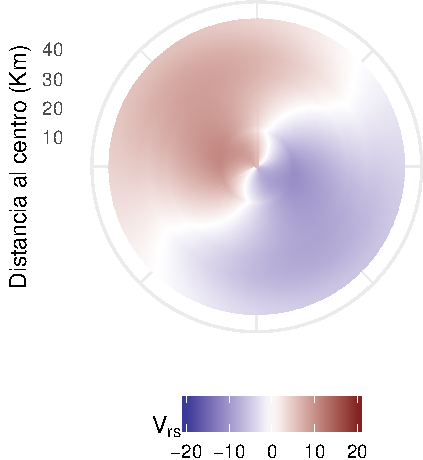
\includegraphics[ ]{Tesis_files/figure-latex/validacion-2} }\newline\subfloat[Con errores \label{ce}\label{fig:validacion3}]{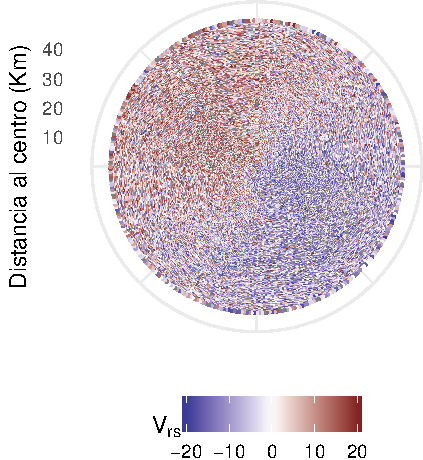
\includegraphics[ ]{Tesis_files/figure-latex/validacion-3} }\subfloat[Con errores + NAs \label{na}\label{fig:validacion4}]{\includegraphics[ ]{Tesis_files/figure-latex/validacion-4} }

}

\caption{Velocidad radial (m/s) observada a las 12 UTC por el radar de Anguil en la elevación $1.3^{\circ}$ y la misma variable transformada a partir del sondeo de la estación Santa Rosa Aero para la misma hora \label{validacion}}\label{fig:validacion}
\end{figure}

En la Figura \ref{validacion} se puede observar el campo de \(V_r\)
observado por el radar (a) y el campo de \(V_{rs}\) obtenidos a partir
del sondeo (b). Cualitativamente se observa que tanto la magnitud como
la dirección del viento son similares pero también que el \(V_rs\) cubre
totalmente el dominio mientras que la señal del \(V_r\) se extingue a
los 15 km de rango. Cuantitativamente la diferencia \(V_r - V_{rs}\) es
grande en puntos localizados pero el error absoluto medio es de 2.08
m/s, un valor razonable teniendo en cuenta que las observaciones son
realizadas por instrumentos distintos.

\begin{itemize}
\tightlist
\item
  \textbf{Con errores aleatorios (EA)}
\end{itemize}

Para realizar una validación más realista se agregaron errores
aleatorios al campo de \(V_{rs}\), esto además permite analizar la
sensibilidad del algoritmo a este tipo de errores.

El nuevo campo perturbado será:

\begin{equation} \label{eq-vr12}
V_{rs}'  = V_{rs} + \alpha \varepsilon(0,1)
\end{equation}

Donde \(\alpha\) es la amplitud del error y \(\varepsilon\) es un número
aleatorio con distribución normal, \(\mu = 0\) y \(\sigma= 1\).

En la Figura \ref{ce} se muestra el campo resultante utilizando
\(\alpha = 1 m/s\), rápidamente se ve la variabilidad impuesta y también
la disminución en la coherencia horizontal aunque se mantiene
aproximadamente el signo de la variable en las distintas regiones.

\begin{itemize}
\tightlist
\item
  \textbf{Con errores aleatorios y datos faltantes (EA+NA)}
\end{itemize}

Otro problema importante en los datos de radar es la ausencia de señal,
esto se ve como datos faltantes (NAs). Para analizar el efecto de los
datos faltantes se aplicó una máscara de NAs al campo de \(V_{rs}'\) de
tal manera que sean los mismo NAs presentes en el volumen de datos de
radar utilizados para que la distribución de Nas sea realista (Figura
\ref{na}).

\subsubsection{Perfiles obtenidos}\label{perfiles-obtenidos}

En la Figura \ref{validacion-perfiles} se muestra el perfil del sondeo
para los primeros 3 km de altura, los perfiles calculado con VAD a
partir de los distintos campos sintéticos y en negro se muestra el
perfil vertical obtenido a partir de las observaciones del radar para
esa hora. En cuanto a la magnitud no se ven diferencias importantes
entre el sondeo y los perfiles sintéticos. Al observar el detalle de los
primeros 1000 metros de altura, la diferencia es menor a 0.5 m/s en
todos los casos. Tampoco se observó sensibilidad al aumento de la
amplitud de error (no se muestra).

\begin{figure}
\includegraphics[ ]{Tesis_files/figure-latex/validacion-perfiles-1} \caption{Viento medio (m/s) en función de la altura a partir del sondeo, y las distintas pruebas de validación a la izquierda y el detalle ampliado del máximo en niveles bajos \label{validacion-perfiles}}\label{fig:validacion-perfiles}
\end{figure}

\begin{longtable}[]{@{}lrr@{}}
\caption{Errores calculados para las distintas pruebas de validación.
\label{validacion-errores}}\tabularnewline
\toprule
Prueba & rms & rre\tabularnewline
\midrule
\endfirsthead
\toprule
Prueba & rms & rre\tabularnewline
\midrule
\endhead
SE & 0.1613 & 0.0194\tabularnewline
EA & 0.3020 & 0.0364\tabularnewline
EA+NA & 0.1778 & 0.0214\tabularnewline
\bottomrule
\end{longtable}

\newpage

Esto puede verificarse con el cálculo de distintos errores (Gao y
Droegemeier, 2004): la raíz del error cuadrático medio
(\(rms = \sqrt{ \frac{\sum (V-V_{ref})^2}{N} }\)) y el error relativo al
rms (\(rre = \sqrt{ \frac{\sum (V-V_{ref})^2}{\sum (V_{ref})^2} }\))
donde \(V_{ref}\) corresponde a la variable de referencia, en este caso
el sondeo. Los resultados se muestran en la Tabla
\ref{validacion-errores} y como puede observarse no hay un aumento
importante al incorporar errores aleatorios y disminuye al quitar datos
en la prueba EA+NA ya que los errores calculados son sensibles a la
cantidad total de datos.

El efecto más importante en las pruebas de validación corresponde a la
presencia de NAs. La falta de datos en distintas regiones para rangos a
partir de 10 a 15 km impide el cálculo del perfil por encima de 800
metros (con excepción de un punto a los 2000 metros de altura).

Si se compara cualitativamente los perfiles de viento obtenidos con el
sonde y el perfil calculado con VAD a partir de los datos de radar se
observa que estos no coinciden. Además de la falta de datos por encima
de los 800 m (debido a la débil señal del radar), la magnitud del viento
observado por el radar es siempre menor y con una diferencia de hasta 2
m/s. Tampoco se observa una similitud en la forma de los perfiles pero
puede deberse, en parte, a los pocos datos disponibles.

\subsection{Configuración del algoritmo
elegida}\label{configuracion-del-algoritmo-elegida}

En la Tabla \ref{parametros} se detallan los valores utilizados en los
distintos parámetros necesarios para el algoritmo VAD que se mantuvieron
para todos los casos de estudio.

\begin{table}

\caption{\label{tab:parametros}Parámetros utilizados en el cálculo del VAD y la construcción de la grilla vertical para todos los casos. \label{parametros}}
\centering
\begin{tabular}[t]{lll}
\toprule
Algoritmo & Parámetro & Valor\\
\midrule
 & Ángulo mínimo & 1.3°\\
\cmidrule{2-3}
 & Ángulo máximo & 11.8°\\
\cmidrule{2-3}
 & Radio interior & 0.3 km\\
\cmidrule{2-3}
 & Radio exterior & 40 km\\
\cmidrule{2-3}
 & NaN máximo & 72\\
\cmidrule{2-3}
 & Gap máximo & 30\\
\cmidrule{2-3}
 & Pesos & -\\
\cmidrule{2-3}
\multirow{-8}{*}{\raggedright\arraybackslash VAD} & R cuadrado & 0.8\\
\cmidrule{1-3}
 & Altura mínima & 0.1 Km\\
\cmidrule{2-3}
 & Altura máxima & 3 Km\\
\cmidrule{2-3}
\multirow{-3}{*}{\raggedright\arraybackslash Grilla vertical} & Espaciado & 0.1 Km\\
\bottomrule
\end{tabular}
\end{table}

\section{Consistencia temporal de las
observaciones}\label{consistencia-temporal-de-las-observaciones}

Ya que uno de los objetivos de esta tesis es estudiar la evolución del
viento a lo largo del día, es importante asegurar cierta consistencia
temporal en los datos. La inconsistencia temporal puede deberse a que
cada volumen de datos no es medido de manera instantánea si no que
demora algunos minutos. Si bien en periodos sin cambios sinópticos
importantes no se espera variaciones bruscas del viento, es posible que
variaciones menores a los 10 minutos (resolución temporal de los datos
de radar) estén afectando la consistencia temporal.

Para solucionar este problema se aplicó un suavizado pesado localmente o
LOWESS (LOcally WEighted Scatterplot Smoothing, Cleveland (1979)).
LOWESS es un método de regresión no paramétrica y por lo tanto no es
necesario asumir que los datos tienen algún tipo de distribución
particular. Esto lo hace un método flexible al representar el
comportamiento de los datos. Por otro lado la estimación para cada punto
se realiza utilizando la información de datos vecinos. Para esto se
especifica cuantos datos vecinos se utilizaran para estimar cada punto
local como una fracción del total de datos.

En la Figura \ref{lowess} se muestra la variación de la velocidad del
viento con el tiempo a 500 m de altura donde se identifican dos momentos
donde la variación del viento da saltos bruscos, alrededor de las 03 y
las 08 UTC. Al aplicar el LOWESS el resultado es un suavizado de la
variable que elimina los saltos bruscos y mejora la coherencia.

\begin{figure}

{\centering \includegraphics{Tesis_files/figure-latex/lowess-1} 

}

\caption{Velocidad del viento a lo largo del tiempo para el 14 de enero de 2016 a 500 m de altura (negro) y la misma variable luego de la aplicación del LOWESS (color). \label{lowess}}\label{fig:lowess}
\end{figure}

\section{Procesos asociados a la CLP}\label{procesos-asociados-a-la-clp}

El estudio de los procesos que ocurren en la CLP es un desafío cuando no
se cuenta con datos de la turbulencia. En esta tesis se abordan procesos
que pueden ser estudiados a partir de los perfiles de viento y las
variables de superficie.

\subsection{Determinación del estado de la
turbulencia}\label{determinacion-del-estado-de-la-turbulencia}

El número de Richardson puede ser utilizado como un estimador de la
estabilidad dinámica (Stull, 1988) y por lo tanto de la turbulencia
presente. Su definición surge como el cociente de los términos de
producción mecánica y térmica de la turbulencia en la ecuación de
energía cinética turbulenta de un fluido gaseoso (Stull, 1988). A partir
de suponer válida la teoría K (Pasquill y Smith, 1983) y que los
coeficientes de intercambio turbulento de calor sensible y de cantidad
de movimiento son iguales, es posible escribir el número de Richardson
en función de los gradientes verticales de viento y temperatura
potencial:

\begin{equation} \label{eq-ri1}
R_i = \frac{\frac{g}{\overline{\theta_v}} \frac{\partial \overline{\theta_v}}{\partial z}}
{\left [ \left (\frac{\partial \overline{u}}{\partial z} \right )^2 + \left (\frac{\partial \overline{v}}{\partial z} \right )^2  \right]}
\end{equation}

El signo de este número permite clasificar la evolución de la
turbulencia en dos clases: estables (\(R_i\) \textgreater{} 0) e
inestables (\(R_i\) \textless{} 0). El numerador de la Ecuación da
cuenta de la disponibilidad de energía asociada a procesos de empuje
térmico que favorecen la destrucción o inhiben la turbulencia en
condiciones estables y la producen en condiciones inestables. El
denominador corresponde a la producción mecánica o por cortante. De
acuerdo a Stull (1988) la turbulencia puede mantenerse si \(R_i\) es
menor a un valor umbral (\(R_T\)), ya que por encima de este umbral (en
general \(R_T = 1\)), la inhibición de la turbulencia se incrementa
tendiendo a estabilizar el estado del flujo y volverlo laminar.

Debido a que la estimación de los gradientes suele ser difícil, estos
tienden a ser expresados en términos de observaciones discretas. Surge
así el número de Richardson Bulk:

\begin{equation} \label{eq-ri2}
R_b = \frac{g \, \Delta \overline{\theta_v} \, \Delta z}{\overline{\theta_v} \, [(\Delta \overline{u}^2) + [(\Delta \overline{v}^2)]}
\end{equation}

Para obtener el \(R_b\) en cada tiempo y su variación con la altura es
necesario contar con el perfil vertical de temperatura virtual
(\(\theta_v\)) y de la velocidad del viento. Debido a que solo se cuenta
con el valor de la temperatura en superficie, se utilizó la siguiente
aproximación válida para estimar el número de Richardson en el periodo
estable:

\begin{equation} \label{eq-ri3}
R_i \sim \frac{(g  \: (\theta_i - \theta_f)/z_{máx})}{(\overline{\theta} \: (u_{máx}/z_{máx})^2)}
\end{equation}

Donde \(\theta_i\) corresponde al valor de la temperatura virtual en
superficie en el momento de transición entre la capa mezclada y el
comienzo de la capa estable nocturna, por lo tanto será la temperatura
en el tope de la capa estable asumiendo que la capa residual no se
modifica. El valor de \(\theta_f\) será la temperatura en superficie
observado. Por último \(u_{máx}\) es el valor máximo de viento observado
y \(z_{máx}\), la altura a la que ocurre este máximo y que se
considerará en este trabajo como una aproximación de la altura del tope
de la capa estable (Ver Sección \ref{sec-pbh}).

\subsection{\texorpdfstring{Altura de la capa límite
\label{sec-pbh}}{Altura de la capa límite }}\label{altura-de-la-capa-limite}

La altura de la capa límite se define como la altura a la cual las
características de la superficie no afecta la atmósfera. Las
estimaciones de esta variable son muy diversas en la literatura y
también sus aplicaciones a los modelos numéricos.

Por ejemplo la altura de la capa estable nocturna puede definirse como
la altura a la cual la intensidad de la turbulencia es una fracción del
valor en superficie mientras que la altura de la capa mezclada puede
determinarse como la altura a la que se observa el menor transporte
vertical de calor sensible.

Teniendo en cuenta los datos disponibles se determinó la altura de la
capa estable nocturna como la altura a la que ocurre el máximo de
viento.

Otro enfoque posible es el uso de la reflectividad. Por ejemplo Kaufmann
y White (1997) buscó determinar la altura a la que ocurre la inversión
térmica en invierno utilizando radares y otros instrumentos asociados
utilizando la variable SNR (Signal to Noise Ratio o relación entre la
Señal y el Ruido de la reflectividad). Por otro lado Chandra et~al.
(2010) utiliza la variación de la reflectividad con la altura observada
con un perfilador radar de viento en casos de aire claro y cielo nuboso.
Esta técnica se basa en el concepto de que en el tope de la capa límite
se observan importantes gradientes de temperatura y humedad y estos
generan un máximo local en la reflectividad. En este trabajo se exploró
de manera preliminar la posibilidad de determinar la altura de la capa
límite a partir de las variación es de la reflectividad observada por el
radar con la altura.

\subsection{Descripción del LLJ}\label{descripcion-del-llj}

El Jet nocturno de capas bajas o LLJ (Low Level Jet) es un fenómeno de
mesoescala caracterizado por por una corriente fuerte de viento con
máximos de entre 10 y 20 m/s que se localiza en los primeros cientos de
metros de altura (Stull, 1988). Su extensión vertical es poca pero
horizontalmente puede extenderse por cientos de kilómetros.

Existen distintos criterios para identificar el LLJ. En algunos casos se
determina un umbral mínimo para la velocidad del viento a partir del
cual se considera la existencia del LLJ siempre que este ocurra por
debajo de algún nivel o altura determinada. En otros casos, se busca que
el viento sea supergeostrófico. En este trabajo se utilizará el criterio
de Bonner (1968) que identifica el LLJ cuando el máximo del viento es
superior a 12 m/s y decrece al menos 6 m/s hasta el próximo mínimo o
hasta el nivel de 3 km.

El LLJ puede producirse por distintos mecanismos entre los que se pueden
nombrar la topografía, baroclinicidad asociada a pendientes del terreno,
frentes y oscilaciones inerciales. En algunas situaciones, varios
mecanismos pueden contribuir a la formación del LLJ de manera conjunta y
estos son los que determinan las características del fenómeno.

En este trabajo el análisis se centra en el LLJ generado por la
oscilación inercial. De acuerdo a Blackadar (1957) luego del atardecer,
cuando no hay producción de turbulencia de origen térmico se produce un
desacople de la capa mezclada y el viento tiende a acelerarse ante la
ausencia de la fricción hacia el equilibrio geostrófico. Sin embargo la
fuerza de Coriolis genera una oscilación inercial del viento alrededor
del viento geostrófico produciendo un LLJ supergeostrófico durante el
periodo estable.

Posteriormente Van de Wiel et~al. (2010) generaliza el modelo de
Blackadar para incluir el efecto de la fricción de superficie (efecto
que no puede ser despreciado dentro de la capa límite) y como resultado
la oscilación del viento ocurre alrededor de un perfil de equilibrio en
vez del viento geostrófico.

De acuerdo al modelo la oscilación puede verse en la rotación del vector
del viento a lo largo del tiempo generando una hodógrafa en forma de
``herradura'' (Baas et~al., 2012). Para el hemisferio sur la rotación
del viento será en sentido antihorario. El periodo de la oscilación
inercial es de \(P = 2\pi/f\), con \(f\) el parámetro de Coriolis. A la
latitud de Paraná \(P = 17.79\) horas y por lo tanto se espera que el
máximo viento ocurra para cuando se alcanza la mitad del periodo desde
el atardecer (Kallistratova y Kouznetsov, 2012).

\section{Modelo WRF}\label{modelo-wrf}

En este trabajo se utilizó el modelo WRF versión 3.9.1 para la
realización de simulaciones numéricas que permitan comparar algunas de
las parametrizaciones de CLP disponibles: YSU (Yonsei University
Scheme), MYJ(Mellor--Yamada--Janjic) y ACM2 (Asymmetric Convection Model
2).

Las simulaciones se integraron en un dominio 1 anidado con un dominio 2
en dos direcciones. El dominio 1 se configuró con una resolución de 12 x
12 km y 105 x 105 puntos de grilla y dominio 2 con una resolución de 4 x
4 km y 253 x 253 puntos de grilla, ambos centrados en la ubicación del
radar de Paraná. Como se puede ver en la Figura \ref{dom-modelo} el
dominio abarca todo el centro y norte del país. Se utilizaron datos
geográficos con 10 minutos de resolución para el dominio superior y 2
minutos para el dominio inferior.

Ambos dominios tienen una grilla vertical de 42 niveles expresados en
coordenadas sigma-p, con una distribución hipérbolo tangencial para que
los primeros 20 niveles se ubiquen en los primeros 1800 m. La presión en
el tope del modelo es de 100 hPa. De acuerdo a Shin et~al. (2012) se
determinó que el nivel inferior se ubique en 40 msns para evitar errores
en algunas variables de superficie asociadas a la CLP.

\begin{figure}

{\centering \subfloat[Dominio utilizado en el modelo con resolución de 12 km (dominio exterior) y 4 km (dominio interior. El punto representa la ubicación del radar. \label{dom-modelo}\label{fig:dominio1}]{\includegraphics{Tesis_files/figure-latex/dominio-1} }\hfill\subfloat[Topografía sobre el nivel del terreno respecto de la ubicación del radar. El circulo negro corresponde al dominio de análisis, de 40km de radio y centrado en el radar. \label{dom-radar}\label{fig:dominio2}]{\includegraphics{Tesis_files/figure-latex/dominio-2} }

}

\caption{Dominios utilizados. \label{dominio}}\label{fig:dominio}
\end{figure}

Se realizaron simulaciones para el periodo comprendido en el Caso 1, es
decir, entre las 06 UTC del 13 de enero a las 00 del 15 de enero de 2016
en todos los casos. Las primeras 6 horas de simulación corresponden al
``spin up'' del modelo y las siguientes 36 horas al período de interés
para el análisis. Si bien el estudio se centra en comparar las
observaciones del 14 de enero con las simulaciones, es importante tener
en cuenta que la capa estable nocturna puede ser muy influenciada por la
capa mezclada del día anterior, por esta razón la simulación empieza 12
horas antes.

Para las condiciones iniciales para las 06 UTC del 13 de enero de 2016
se utilizó el Análisis Final (FNL) de National Centers for Environmental
Prediction (NCEP) con resolución de 0.25° X 0.25° y las condiciones de
borde fueron forzadas por los mismos datos cada 6 horas.

Para los procesos físicos no asociados a la CLP se usaron las siguientes
parametrizaciones: RRTMG (Rapid Radiative Transfer Model for GCMs,
Mlawer et~al. (1997)) para la radiación de onda larga, Dudhia (Dudhia,
1989) para la radiación de onda corta, WSM6 (WRF Single-Moment 6-Class
Microphysics, Hong y Lim (2006)) para los procesos microfísicos, el
esquema Kain-Fritsch para los procesos de convección y el modelo Noah de
superficie (Tewari et~al., 2016).

\subsection{Parametrizaciones de capa
límite}\label{parametrizaciones-de-capa-limite}

Se presentan las características generales de cada parametrización
analizada y el esquema de capa de superficie asociado a cada una (ya que
cada parametrización de CLP tiene una determinada parametrización de
capa de superficie y lamentablemente no se puede utilizar una en común).

\begin{itemize}
\tightlist
\item
  \textbf{YSU}
\end{itemize}

El esquema YSU (Hong et~al., 2006) es un esquema no local y como
previamente se mencionó, determina el valor de una variable no conocida
en un punto a partir de variables conocidas en distintos puntos. Está
configurado con una clausura de primer orden y considera la mezcla no
local debido a torbellinos grandes agregando un término de ajuste de
gradiente al gradiente local a cada variable de pronóstico. El esquema
usa la parametrización de capa de superficie MM5 Monin-Obukohv
Similarity.

\begin{itemize}
\tightlist
\item
  \textbf{MYJ}
\end{itemize}

El esquema MYJ es un esquema local que usa una clausura de orden 1.5 y
determina los coeficientes de difusión a partir del cálculo de la
energía cinética de las perturbaciones pronosticada (Janjić, 1994). MYJ
usa el esquema de capa de superficie Janjic Eta Monin--Obukhov.

\begin{itemize}
\tightlist
\item
  \textbf{ACM2}
\end{itemize}

Este esquema es similar a YSU en el sentido de que es no local y tiene
clausura de primer orden. Sin embargo considera un transporte no local
hacia arriba y un transporte local hacia abajo ``capa a capa'' para las
variables de pronóstico (Pleim, 2007). También utiliza el esquema de
capa de superficie MM5 Monin-Obukohv Similarity.

\subsection{Procesamiento de los
datos}\label{procesamiento-de-los-datos}

Las simulaciones fueron post procesadas con el módulo ARWPost donde se
eligió una resolución vertical de 100 metros en los primeros kilómetros
de la atmósfera de tal manera que coincida con la grilla vertical de las
observaciones de radar. El dominio inicial fue recortado para analizar
el disco de 40 km de radio alrededor del radar como se muestra en la
Figura \ref{dom-radar}.

El análisis del viento requiere un segundo procesamiento para
transformar la variable a la grilla del radar y de esta manera obtener
el perfil vertical de viento a partir del VAD y de esa manera, mejorar
la comparación con las observaciones. Este procesamiento se realiza con
la librería LETKF-WRF (Ruiz y Mandonado, 2017) a partir de las salidas
no procesadas del modelo.

El análisis del resto de las variables pueden hacerse tomando el dato
del punto más cercano al radar o a partir del promedio espacial en todo
el dominio analizado. Se explorarán ambas posibilidades para determinar
posibles diferencias y analizar la homogeneidad espacial de las
variables.

\subsection{Tratamiento de variables asociadas a la
CLP}\label{tratamiento-de-variables-asociadas-a-la-clp}

Fue posible configurar el modelo para obtener algunas variables
específicas de los esquemas de CLP como la altura de la capa límite
estimada por cada parametrización (\(h\)), la Longitud de Monin-Obukohv
(\(L\)), la velocidad de fricción (\(u_*\)) y el coeficiente de
difusividad de calor (\(K_h\)).

\subsubsection{Estimación de la altura de la
CLP}\label{estimacion-de-la-altura-de-la-clp}

Si bien cada parametrización estima la altura de la CLP, esta estimación
es distinta en cada esquema. YSU calcula el número de Richarson Bulk
desde superficie y determina \(h\) como la altura a la cual \(R_b\)
alcanza un valor cŕitico: cero para el régimen inestable y 0.25 para el
regimen estable (Hong et~al., 2006). ACM2 utiliza el mismo valor crítico
del \(R_b\) pero en los casos inestables el cálculo del número de
Richarson se realiza para la capa de entremezcla entre la CLP y la
atmósfera libre (Pleim, 2007). Por otro lado el esquema MYJ diagnostica
la altura de la CLP como la altura a la cual la energía cinética
turbulenta alcanza un valor prescripto en \(0.1 m^2/s^2\) (Janjić,
1994).

Esto hace que la comparación entre las distintas parametrizaciones no
sea del todo válida. Por esta razón además de utilizar el valor de \(h\)
para cada parametrización, en el caso de la capa estable nocturna se
estimará la altura de la capa a partir de la altura a la que ocurre el
máximo de viento siguiendo la metodología utilizada para la
observaciones (Sección \ref{sec-pbh}) y realizar una mejor comparación.

\subsubsection{Coeficientes de difusividad
turbulenta}\label{coeficientes-de-difusividad-turbulenta}

Si bien se obtuvo el valor de \(K_h\) para cada punto de grilla y cada
tiempo, no fue posible obtener el coeficiente de difusividad de cantidad
de movimiento (\(K_m\)) directamente desde el modelo por lo que se
estimó a partir de la relación \(K_m = K_h \: P_r\) donde \(P_r\) es el
número de Prandtl. Este último se determinó calculando los perfiles de
los coeficientes de difusividad según Ulke (2000):

\begin{itemize}
\tightlist
\item
  \textbf{Condiciones estables (\(h/L > 0\))}
\end{itemize}

\begin{equation} \label{k-1}
K_m(z) =  ku_{*o}h\left (\frac{z}{h} \right )\left(1-\frac{z}{h} \right)\left (1 + 6.9\frac{h}{L}\frac{z}{h} \right)^{-1}
\end{equation}

\begin{equation} \label{k-2}
K_h(z) =  ku_{*o}h\left (\frac{z}{h} \right )\left(1-\frac{z}{h} \right)\left (1 + 9.2\frac{h}{L}\frac{z}{h} \right)^{-1}
\end{equation}

\begin{itemize}
\tightlist
\item
  \textbf{Condiciones inestables (\(h/L < 0\))}
\end{itemize}

\begin{equation} \label{k-3}
K_m(z) =  ku_{*o}h\left (\frac{z}{h} \right )\left(1-\frac{z}{h} \right)\left (1 - 22\frac{h}{L}\frac{z}{h} \right)^{1/4}
\end{equation}

\begin{equation} \label{k-4}
K_h(z) =  ku_{*o}h\left (\frac{z}{h} \right )\left(1-\frac{z}{h} \right)\left (1 - 13\frac{h}{L}\frac{z}{h} \right)^{1/2}
\end{equation}

donde \(u_*\) es la velocidad de fricción y \(k\) la constante de Von
Karman. A partir de este modelo se obtiene \(P_r(z) = K_m/K_h\) para
obtener el coeficiente de difusividad de cantidad de movimientos a
partir de los datos del modelo.

\chapter{Resultados}\label{resultados}

\section{Descripción de los casos de
estudio}\label{descripcion-de-los-casos-de-estudio}

A partir de los criterios establecidos en la Sección \ref{sec-criterios}
se identificaron tres casos de estudio cuyas características principales
se describen a continuación.

\subsection{Caso 1: 14 de enero de
2016}\label{caso-1-14-de-enero-de-2016}

El caso 1 abarca el periodo de las 00 UTC del 14 de enero a las 00 UTC
del 15 de enero de 2016. De acuerdo a la Figura \ref{hgt-caso1} donde se
muestra la altura geopotencial en 1000 hPa para dos momentos, se observó
un anticiclón ubicado sobre el océano Atlántico y al este Uruguay a las
00 UTC de 14 de enero. Este sistema está asociado a vientos del norte
sobre el dominio en estudio. En superficie se registraron vientos
débiles (menores a 2 m/s) del este y sureste en las primeras horas del
periodo. En la estación meteorológica se observó nubosidad en niveles
altos en las primeras horas de tipo \emph{cirrostratus} que por momentos
cortos cubrió parcialmente el cielo. No se observaron ecos
meteorológicos en la región del radar. Si bien la presencia de nubosidad
puede afectar la evolución de la capa límite en este caso no se observan
variaciones en la temperatura fuera de lo normal para cada momento del
período (Figura \ref{meteo1}).

Posteriormente, a las 12 UTC el anticiclón se intensificó y comenzó a
moverse hacia el NE mientras que en superficie se observaron vientos
predominantes del noreste de hasta 6.5 m/s. No se observó nubosidad y la
temperatura en superficie alcanzó los 32.4°C. El aumento de humedad
específica observado alrededor de las 12 UTC coincidió con el el momento
donde se registraron vientos del sector norte y noreste.

\begin{figure}

{\centering \includegraphics{Tesis_files/figure-latex/hgt-caso1-1} 

}

\caption{Altura geopotencial en 1000 hPa para las 00 y las 12 UTC del 14 de enero de 2016 (Caso 1). Datos de Reanálisis NCEP (NOAA/OAR/ESRL PSD - Kalnay et al., 1996). \label{hgt-caso1}}\label{fig:hgt-caso1}
\end{figure}

\begin{figure}

{\centering \includegraphics{Tesis_files/figure-latex/meteo-caso1-1} 

}

\caption{Variables de superficie observadas por la estación meteorológica Paraná el 14 de enero de 2016. La región sombreada corresponde a al período donde se observa nubosidad (ver texto). Datos Servicio Meteorológico Nacional. \label{meteo1}}\label{fig:meteo-caso1}
\end{figure}

\subsection{Caso 2: 21 de enero de
2016}\label{caso-2-21-de-enero-de-2016}

El caso 2 comprende el período entre las 00 UTC del 21 de enero a las 00
UTC del 22 de enero de 2016. A escala regional a las 00 UTC (Figura
\ref{hgt-caso2}) se observó un anticiclón ubicado sobre el océano
Atlántico frente a la costa de Argentina, mientras que en el centro del
país se observó una región de baja presión. De acuerdo a los datos de la
estación meteorológica en las primeras horas del día el viento estuvo en
calma y llegando a los 2 m/s en algunos momentos. La dirección
predominante fue del E y SE en algunas horas. En cuanto a la nubosidad,
en las primeras cuatro horas se observó nubosidad de tipo
\emph{cirrostratus} que no cubrió la totalidad del cielo en ningún
momento. No no afectó el descenso de temperatura durante las horas
nocturnas (Figura \ref{meteo2}).

Posteriormente a las 12 UTC del mismo día el anticiclón se debilitó y se
desplazó hacia el noreste. El viento en superficie fue de predominante
del N a partir de esa hora con máximos de hasta 5.5 m/s. Esta situación
generó un aumento de la humedad específica proveniente del norte con un
máximo luego de las 14 UTC. Entre las 09 y las 16 UTC se observó
nubosidad tipo \emph{cirro} que no llegó a cubrir la totalidad del
cielo. Esta nubosidad no afectó de manera observable la temperatura en
superficie que llegó a 35.4°C. En las observaciones del radar no se vió
nubosidad en las inmediaciones.

\begin{figure}

{\centering \includegraphics{Tesis_files/figure-latex/hgt-caso2-1} 

}

\caption{Altura geopotencial en 1000 hPa para las 00 y las 12 UTC del 21 de enero de 2016 (Caso 2). Datos de Reanálisis NCEP (NOAA/OAR/ESRL PSD - Kalnay et al., 1996). \label{hgt-caso2}}\label{fig:hgt-caso2}
\end{figure}

\begin{figure}

{\centering \includegraphics{Tesis_files/figure-latex/meteo-caso2-1} 

}

\caption{Variables de superficie observadas por la estación meteorológica Paraná el 21 de enero de 2016. La región sombreada corresponde a al período donde se observa nubosidad (ver texto). Datos Servicio Meteorológico Nacional. \label{meteo2}}\label{fig:meteo-caso2}
\end{figure}

\subsection{Caso 3: 23 de enero de
2016}\label{caso-3-23-de-enero-de-2016}

El caso 3 abarca el periodo de las 00 UTC del 23 de enero a las 00 UTC
del 24 de enero de 2016. A nivel regional el campo de altura
geopotencial en 1000 hPa mostró una región de baja presión en el centro
del país (Figura \ref{hgt-caso3}) que fue desplazándose hacia el NE a lo
largo del periodo. Esta configuración puede ser asociada con vientos del
N en la región de Paraná, lo que se confirma con los datos de viento
registrados en la estación meteorológica débiles a moderados (entre 1.5
y 5 m/s).

Entre las 06 y 09 UTC se observó nubosidad que cubrió dos octavos del
cielo de tipo \emph{altocumulus} semitransparentes. Si bien esta
nubosidad se observó alejada de radar (a más de 60 km hacia el NE),
puede ser la causa del estancamiento de la temperatura en la estación
meteorológica durante ese período pero que luego siguió descendiendo al
desaparecer la nubosidad. El máximo de humedad específica observado
durante las horas nocturnas pudo deberse al transporte de humedad debido
al viento del N y del NNE (Figura \ref{meteo3}).

A las 12 UTC el centro de baja presión fue reemplazado por un anticiclón
que se ubicó al sur de la provincia del Buenos Aires y sobre la costa
del océano Atlántico. En superficie se registró viento del NO y O con un
máximo de 5.5 m/s). Entre las 14 y las 17 UTC se registró nubosidad alta
de tipo \emph{cirrus} en forma de filamentos y bandas que no cubrieron
la totalidad del cielo en ningún momento. El aumento diurno de la
temperatura fue constante hasta llegar a una máxima de 37.2°C a las 20
UTC.

\begin{figure}

{\centering \includegraphics{Tesis_files/figure-latex/hgt-caso3-1} 

}

\caption{Altura geopotencial en 1000 hPa para las 00 y las 12 UTC del 23 de enero de 2016 (Caso 3). Datos de Reanálisis NCEP (NOAA/OAR/ESRL PSD - Kalnay et al., 1996). \label{hgt-caso3}}\label{fig:hgt-caso3}
\end{figure}

\begin{figure}

{\centering \includegraphics{Tesis_files/figure-latex/meteo-caso3-1} 

}

\caption{Variables de superficie observadas por la estación meteorológica Paraná el 23 de enero de 2016. La región sombreada corresponde a al período donde se observa nubosidad (ver texto). Datos Servicio Meteorológico Nacional. \label{meteo3}}\label{fig:meteo-caso3}
\end{figure}

\section{Análisis de las observaciones de radar procesadas con
VAD}\label{analisis-de-las-observaciones-de-radar-procesadas-con-vad}

\subsection{Magnitud y velocidad del
viento}\label{magnitud-y-velocidad-del-viento}

Los datos de \(V_r\) del radar fueron procesados para obtener la
magnitud y la intensidad del viento para el período correspondiente a
cada caso de estudio. Debido a que la señal de radar en días de aire
claro no supera a los primeros kilómetros de atmósfera y los controles
de calidad impuestos, en muchos tiempos los resultados no alcanzan los
3000 m de altura.

La magnitud y dirección del viento para el Caso 1 se muestra en la
Figura \ref{campo-caso1}. En la Figura \ref{caso1-spd} se puede observar
en contornos la magnitud del viento en función de la altura y a lo largo
del tiempo para todo el período correspondiente al Caso 1 y en símbolos
los errores calculados. Las mayores velocidades de viento se observan en
horas nocturnas con un máximo de 16 m/s cercano a las 06 UTC y a 300
metros de altura. Este máximo comienza a observarse a partir de las 03
UTC y se extiende más allá de las 12 UTC (3 horas después de la salida
del sol). Posteriormente durante el día la magnitud del viento disminuye
a valores del orden de 4 m/s y su variación con la altura es mucho menor
en comparación con las horas previas lo que corresponde a las
características de la capa mezclada. En las últimas horas la velocidad
del viento comienza a aumentar nuevamente con valores de hasta 8 m/s
coincidiendo con la puesta del sol cuando la capa mezclada queda
desacoplada de la superficie y comienza a desarrollarse la capa estable
nocturna.

En el período nocturno se observa un aumento en la magnitud de los
errores, principalmente del \(rmse_2\) que está asociado a un mayor
error en los anillos de datos al estimar el valor del viento en esa
región. Los mayores valores del \(rmse_2\) (hasta 3.8 m/s) se observan
en los bordes de las regiones donde hay datos tanto en niveles altos
como en los niveles inferiores por lo que es posible que por fuera de
estos límites los datos de radar no hayan cumplido con los controles de
calidad y fueron descartados. El \(rmse_1\) asociado a la dispersión de
los datos, es menor a 0.5 m/s para la mayoría de los tiempos y altura.
Algunas excepciones ocurren alrededor de las 08 UTC y para el mismo
volumen de datos.

En la Figura \ref{caso1-dir} se muestra la dirección del viento en
función de la altura y el tiempo, los vectores representan la dirección
y sentido del viento y en colores y largo de cada vector la magnitud. Se
observa que en las primeras horas del Caso 1 es predominante del E y SE
en niveles altos. En horas posteriores se observa una rotación mostrando
vientos del NE durante el máximo nocturno. Durante el día el viento se
mantiene con dirección N y NE. El nivel más bajo corresponde a los datos
de viento observados en la estación meteorológica, si bien no se observa
mucha coherencia, esto puede deberse al origen de los datos o
diferencias en la ubicación geográfica.

\begin{figure}
\subfloat[Magnitud del viento. \label{caso1-spd}\label{fig:campo-caso11}]{\includegraphics{Tesis_files/figure-latex/campo-caso1-1} }\newline\subfloat[Dirección. \label{caso1-dir}\label{fig:campo-caso12}]{\includegraphics{Tesis_files/figure-latex/campo-caso1-2} }\caption{Magnitud y dirección del viento  correspondiente al Caso 1 (14/01/2016) observados por el radar y procesados con VAD. En el caso de la magnitud del viento se muestran los errores calculados ($rmse_1$ en círculos y $rmse_2$ en cruces) cuando superan los 0.5 m/s. \label{campo-caso1}}\label{fig:campo-caso1}
\end{figure}

La Figura \ref{campo-caso2} muestra la evolución del viento a lo largo
del tiempo y para cada altura en el Caso 2. En la Figura \ref{caso2-spd}
se puede observar que la magnitud del viento presenta características
similares a las observadas en el análisis del Caso 1. Durante las horas
nocturnas se observa un máximo de viento que llega a los 15 m/s que
comienza a formarse antes de las 03 UTC y persiste luego de las 12 UTC.
A diferencia del Caso 1, en este caso las velocidades altas se extienden
por encima de los 1000 metros de altura. En las horas diurnas la
velocidad del viento disminuye a valores menores a 7 m/s y hay muy poca
variación con la altura llegando a ser constante entre las 16 y las 19
UTC por debajo de los 1500 metros. Lamentablemente no hay suficientes
datos disponibles para las últimas horas del día pero puede apreciarse
un ligero aumento de la velocidad signo del incipiente desarrollo de la
capa estable nocturna.

Los errores calculados presentan un patrón similar a lo observado en el
Caso 1. Predomina el \(rmse_2\) asociado al error relativo cometido en
el ajuste de los datos de radar en los bordes entre la región con y sin
datos. Es importante notar que en algunos casos este error llega a tener
una magnitud de 4 m/s donde la velocidad del viento es de entre 4 y 7
m/s, por lo que la estimación de la magnitud del viento en esas regiones
no es buena y debe analizarse con cuidado. En este caso hay errores y
regiones sin datos en niveles bajos y por encima de los 1500 m durante
el día, lo que dificulta el análisis de la capa mezclada.

La dirección del viento se nuestra en la Figura \ref{caso2-dir}, donde
puede apreciarse la falta de datos en algunos momentos de la tarde. En
la primeras horas de la noche el viento es del NE y luego rota hacia el
N pero se mantiene del NE en los niveles donde se observa el máximo de
viento. En niveles altos el viento es del NO y O. A las 02 UTC los datos
de los primeros niveles no son consistentes con los datos de niveles
superiores o tiempos cercanos, esto puede deberse a un problema con los
datos de radar ya que también tienen asociado un error relativo en la
magnitud del viento. Durante el día el viento predominante es del N y
esto coincide con el viento observado en la estación meteorológica para
esas horas.

\begin{figure}
\subfloat[Magnitud del viento. \label{caso2-spd}\label{fig:campo-caso21}]{\includegraphics{Tesis_files/figure-latex/campo-caso2-1} }\newline\subfloat[Dirección. \label{caso2-dir}\label{fig:campo-caso22}]{\includegraphics{Tesis_files/figure-latex/campo-caso2-2} }\caption{Magnitud y dirección del viento  correspondiente al Caso 2 (21/01/2016) observados por el radar y procesados con VAD. En el caso de la magnitud del viento se muestran los errores calculados ($rmse_1$ en círculos y $rmse_2$ en cruces) cuando superan los 0.5 m/s. \label{campo-caso2}}\label{fig:campo-caso2}
\end{figure}

Finalmente la evolución de la magnitud y la dirección del viento con el
tiempo y la altura para el Caso 3 se muestra en la Figura
\ref{campo-caso3}. La magnitud del viento (Figura \ref{caso3-spd})
presenta características similares a los casos anteriores ya que se
observa un máximo de viento en las horas nocturnas pero con algunas
particularidades. En primer lugar el máximo se desarrolla de las 00 UTC
y persiste (con algunas intermitencias) pasadas las 14 UTC. En segundo
lugar el máximo de viento cambia de nivel con el paso de las horas.
Inicialmente se encuentra a 300 m y con una magnitud de 15 m/s, luego
asciende a 400 m con la misma magnitud y finalmente, luego de disminuir
su intensidad reaparece a los 500 m con una magnitud de 11 m/s. Este
último máximo que ocurre alrededor de las 12 UTC, casi 3 horas después
del amanecer y por esto podría no estar asociado a los procesos que
ocurren en la capa estable nocturna y que dan lugar a los máximos
descriptos previamente. Este máximo secundario afecta la evolución de la
capa límite durante el día pero sin embargo se observa una disminución
del viento que llega a ser casi constante luego de las 15 UTC. No hay
suficientes datos luego de las 18 UTC para determinar la evolución de la
capa mezclada al finalizar el día.

El \(rmse_2\) de la magnitud del viento en este caso es menor a los
casos anteriores (menores a 2.5 m/s) pero también marcan el límite donde
los datos dejan de ser confiables al punto de ser eliminados por los
controles de calidad del algoritmo. A diferencia de las otras
situaciones, hay una región marcada donde el \(rmse_1\) tiene magnitud
por encima de 0.5 m/s que se ubica en niveles por encima del máximo de
viento y entre las 04 y las 08 UTC. Esto puede analizarse como una
región donde los valores de viento estimados por los datos de radar en
cada nivel tienen mucha dispersión. Si bien esto es importante, los
errores son inferiores a 1.7 m/s.

La dirección del viento (Figura \ref{caso3-dir}) presenta
características particulares, en términos generales predomina el viento
del O y NO aunque en los primeros 1000 m y durante la noche el viento es
del N y en niveles altos el viento rota con dirección SO. Durante el día
el viento es principalmente del O.

\begin{figure}
\subfloat[Magnitud del viento. \label{caso3-spd}\label{fig:campo-caso31}]{\includegraphics{Tesis_files/figure-latex/campo-caso3-1} }\newline\subfloat[Dirección. \label{caso3-dir}\label{fig:campo-caso32}]{\includegraphics{Tesis_files/figure-latex/campo-caso3-2} }\caption{Magnitud y dirección del viento  correspondiente al Caso 3 (23/01/2016) observados por el radar y procesados con VAD. En el caso de la magnitud del viento se muestran los errores calculados ($rmse_1$ en círculos y $rmse_2$ en cruces) cuando superan los 0.5 m/s. \label{campo-caso3}}\label{fig:campo-caso3}
\end{figure}

En la Figura \ref{perfiles-horarios} se muestran perfiles verticales del
viento de los 3 casos analizados para dos momentos del día, por la noche
a las 06 UTC y de día a las 17 UTC. Si bien estos datos son mostrados en
las figuras previas, la Figura \ref{perfiles-horarios} permite analizar
la forma de los perfiles verticales. En el caso de los perfiles
nocturnos se observa el máximo de viento en niveles bajos asociado al
LLJ por su forma de ``nariz'' (Banta et~al., 2003; Klein et~al., 2016) y
que luego disminuye en niveles altos a valores típicos de la capa
mezclada diurna. Como se observó previamente el perfil vertical en el
Caso 2 tiene una disminución más lenta con la altura por encima del
máximo.

En los perfiles diurnos característicos de la capa mezclada la magnitud
del viento es aproximadamente nula en superficie aumentando en los
primeros metros para luego mantenerse constante con la altura (Stull,
1988). En estos casos, el nivel más bajo donde se tienen datos
corresponde a las observaciones de la estación meteorológica a 10 m de
altura y por lo tanto no es esperable que se cumpla la primera
característica. Sin embargo se observa un leve aumento de la magnitud
del viento con la altura que a partir de los 100 a 200 metros es casi
nulo dando lugar a un perfil aproximadamente constante. El valor del
\(rmse_2\) que se muestra sombreado es casi despreciable a excepción de
los últimos niveles en los perfiles nocturnos.

\begin{figure}

{\centering \includegraphics{Tesis_files/figure-latex/perfiles-1} 

}

\caption{Perfil de viento observado por el radar a las 06 y las 17 UTC y el $rmse_2$ en cada punto (sombreado) para los tres casos. Las marcas en los ejes indican la magnitud del viento máxima y mínima y la altura a la que ocurren. Los valores en superficie fueron obtenidos a partir de los datos del la estación meteorológica Paraná Aero. \label{perfiles-horarios}}\label{fig:perfiles}
\end{figure}

La variación de la dirección del viento con la altura puede analizarse a
partir de un hodógrafa. En la Figura \ref{hodografa-h} se muestra la
hodógrafa de las 06 UTC para cada caso. El triángulo corresponde al
nivel inferior y los círculos grandes se ubican cada 500 m. De acuerdo
al comportamiento de la espiral de Ekman se espera que la rotación del
viento sea en sentido antihorario dentro de la capa límite. Si bien
existen controversias respecto de la validez de la espira de Ekman en la
capa límite atmosférica (Stull, 1988) se observa en los tres casos una
rotación antihoraria en los primeros metros (correspondientes a la capa
estable nocturna), que se mantiene en todo el perfil para los casos 2 y
3.

\begin{figure}

{\centering \includegraphics{Tesis_files/figure-latex/hodografa-horaria-1} 

}

\caption{Variación del vector del viento en función de la altura entre 100 y 3000 metros, para cada caso de estudio observada por el radar a las 06 UTC. El triángulo marca el nivel inferior y los círculos grandes se ubican cada 500 metros. \label{hodografa-h}}\label{fig:hodografa-horaria}
\end{figure}

\subsection{Características de la capa límite
planetaria}\label{caracteristicas-de-la-capa-limite-planetaria}

\subsubsection{Altura de la capa límite y
turbulencia}\label{altura-de-la-capa-limite-y-turbulencia}

En la Figura \ref{pblh-dbz} se muestra el valor absoluto del gradiente
vertical de reflectividad (\(\nabla_z dBZ\)) medido por el radar en
función de la altura y el tiempo para cada caso de estudio. En días de
aire claro las variaciones de la reflectividad dependen de la
variaciones de la temperatura y humedad en el aire. Estas propiedades
modifican el índice de refracción del aire y producen un aumento en la
variación de la reflectividad con la altura. Es por esto que en las
figuras se buscó resaltar los niveles donde el gradiente vertical de
reflectividad fuera mayor independientemente del signo. Luego de la
exploración de los datos se decidió utilizar sólo los datos del ángulo
de 5° de elevación por tener poco ruido y presentar cierta coherencia
espacial. Sin embargo en los primeros niveles la variación de
\(\nabla_z dBZ\) presenta mucho ruido por lo que no se muestra.

En el Caso 1 (Figura \ref{dbz-1}) se observa un máximo del
\(\nabla_z dBZ\) a aproximadamente 300 m de altura entre las 03 y 9 UTC
que luego se eleva rápidamente y forma dos máximos, uno a 1000 m hasta
las 15 UTC y el otro por encima hasta las 21 UTC. Por las
características, el primer máximo corresponde al tope de la capa estable
y por encima de este hay regiones donde el \(\nabla_z dBZ\) tiene
máximos y que podrían ocurrir debido a la presencia del tope de la capa
residual donde puede existir una importante variación remanente de la
temperatura y la humedad debido a los procesos de mezcla turbulenta
entre la capa mezclada y la atmósfera libre durante el día anterior. En
la segunda mitad del periodo es interesante notar que la altura de los
máximos de \(\nabla_z dBZ\) aumenta rápidamente con el tiempo luego del
amanecer aunque no es posible determinar cuál de los máximos representa
el tope de la capa mezclada.

En la Figura \ref{dbz-2} se muestra el \(\nabla_z dBZ\) para el Caso 2.
Las regiones de máximo gradiente no son tan claras como en el Caso 1
pero es posible determinar una línea entre 500 y 1000 m previo a las 09
UTC que podría corresponder al tope de la capa estable nocturna. Luego
de ese momento, el máximo del gradiente aumenta rápidamente hasta
alcanzar los 1500 m de altura y comienza a descender luego de las 12
UTC. Este comportamiento no es típico de la capa mezclada y podría
deberse a la presencia de nubosidad alta tipo \emph{cirro} que se
observó entre las 09 y las 16 UTC (Figura \ref{meteo2}). Si bien la
marcha de temperatura no parece haber sido afectada por la nubosidad es
posible que el desarrollo de la turbulencia si lo fuera impidiendo el
desarrollo de una capa mezclada más profunda luego de la mitad del día.

La variación de \(\nabla_z dBZ\) con la altura para el Caso 3 se muestra
en la Figura \ref{dbz-3}. Durante la noche en las primeras horas se
observa un máximo cercano a 2000 m que luego desciende y podría
corresponder al tope de la capa residual. Por otro lado se observa por
debajo de 500 m un máximo intenso que se mantiene durante horas hasta
las 14 UTC. Durante la noche este máximo puede asociarse al tope de la
capa estable pero luego del amanecer la persistencia de esta capa de
gran variabilidad en la reflectividad podría deberse a la presencia de
la cortante vertical de viento generada por el máximo de viento
secundario que se observa en la Figura \ref{caso3-spd} a las 12 UTC. Al
igual que en los otros casos se observa un máximo que crece desde las 9
UTC y alcanza rápidamente los 2000 m de altura. Este máximo que se
mantiene durante el día podría deberse al tope de la capa mezclada.

\begin{figure}

{\centering \subfloat[Caso 1. \label{dbz-1}\label{fig:pblh-dbz1}]{\includegraphics{Tesis_files/figure-latex/pblh-dbz-1} }\newline\subfloat[Caso2. \label{dbz-2}\label{fig:pblh-dbz2}]{\includegraphics{Tesis_files/figure-latex/pblh-dbz-2} }\newline\subfloat[Caso 3. \label{dbz-3}\label{fig:pblh-dbz3}]{\includegraphics{Tesis_files/figure-latex/pblh-dbz-3} }

}

\caption{Valor absoluto del gradiente vertical de dBZ en función de la altura y el tiempo. \label{pblh-dbz}}\label{fig:pblh-dbz}
\end{figure}

En la Figura \ref{estable-vad} se muestran algunas características de la
capa estable nocturna asociadas a la turbulencia que pueden estimarse a
partir de los datos disponibles. En primer lugar se estimó la altura de
la capa estable como el nivel en el cual ocurre el máximo viento (Figura
\ref{h-vad}) durante el período donde se observó el máximo. Esta
estimación depende de la resolución vertical elegida para el cálculo del
VAD que en este caso es de 100 m, por lo tanto la estimación no es muy
precisa. En la Figura \ref{cortante-vad} se presenta la cortante
vertical calculada por debajo del máximo del viento y en la Figura
\ref{ri-vad} el número de Richardson calculado de acuerdo a la Ecuación
\ref{eq-ri3} donde los períodos sombreados corresponden a los momentos
donde se observó el máximo de viento y por lo tanto donde estas
aproximaciones son válidas.

En el Caso 1 la altura de la capa estable se mantuvo en 300 m en todo
momento coincidiendo con lo estimado a partir del \(\nabla_z dBZ\). La
cortante de viento tuvo variaciones temporales con un máximo que
coincidió con el momento donde el LLJ fue más intenso. De acuerdo a
(Banta et~al., 2003), estos valores de cortante están asociados a la
presencia de energía cinética turbulenta y podría ser usada como un
estimado de la turbulencia en la capa. Consistente con lo anterior, el
número de Richardson es siempre positivo y por lo tanto estamos ante una
situación de estabilidad estática y además se mantiene por debajo de 1
por lo tanto el flujo se mantiene turbulento debido a procesos mecánicos
asociados a la cortante.

En los Casos 2 y 3 la cortante vertical y el número de Richardson tienen
un comportamiento similar al primer caso y por lo tanto corresponden a
situaciones estables pero donde el flujo es turbulento. Sin embargo a
partir de las 10 UTC en el Caso 3 se observa un aumento en el número de
Richardson que supera el valor crítico \(R_T = 1\) y una disminución de
la cortante, esto implica un incremento en la inhibición de la
turbulencia tendiendo a estabilizar el flujo hasta volverlo laminar.

La estimación del tope de la capa estable en el Caso 2 no coincide con
lo observado en la Figura \ref{dbz-2} ya que de acuerdo a este criterio
se ubica en 200 m. En el Caso 3 las dos estimaciones si coinciden y
además se observa coincidencia en la evolución a lo largo del tiempo.

\begin{figure}
\subfloat[Altura de la capa estable \label{h-vad}\label{fig:estable-vad1}]{\includegraphics{Tesis_files/figure-latex/estable-vad-1} }\newline\subfloat[Cortante ($u_{máx}/z_{máx}$) \label{cortante-vad}\label{fig:estable-vad2}]{\includegraphics{Tesis_files/figure-latex/estable-vad-2} }\newline\subfloat[Número de Richardson \label{ri-vad}\label{fig:estable-vad3}]{\includegraphics{Tesis_files/figure-latex/estable-vad-3} }\caption{Series de tiempo de la altura de la capa límite, cortante vertical y el número de Richarsdon en la capa estable nocturna para todos los casos de estudio. En a) y b) se muestra solo el período donde se observa el LLJ, en c) el período en cada caso se encuentra sombreado. \label{estable-vad}}\label{fig:estable-vad}
\end{figure}

\subsubsection{Oscilación inercial y
LLJ}\label{oscilacion-inercial-y-llj}

Si bien en los perfiles mostrados en la Figura \ref{perfiles-horarios}
se observa claramente las características típicas del LLJ con el máximo
viento en los primeros cientos de metros, el criterio de Bonner permite
detectar el LLJ de manera cuantitativa. De acuerdo al Criterio 1 el LLJ
ocurre si el máximo de viento es igual o superior a 12 m/s y disminuir
al menos 6 m/s en el siguiente mínimo (Bonner, 1968). Valores análogos
se siguen para máximos de mayor magnitud, por ejemplo si el máximo es de
16 m/s, el mínimo tendrá que ser de al menos 8 m/s (Criterio 2). Esto
también puede verse en la Figura \ref{perfiles-horarios} observando la
diferencia entre las marcas verticales en el eje horizontal que
representan el mínimo y el máximo en cada perfil nocturno. En todos los
casos en estudio el criterio de Bonner se cumple satisfactoriamente.

En la Figura \ref{hodografa-n} se muestran hodógrafas para tres niveles
distintos (el primero correspondiente a las observaciones de la estación
meteorológica) desde las 00 UTC. El cuadrado indica el punto final del
vector del viento en el primer tiempo y los círculos grandes,
corresponden al vector en intervalos cada 6 horas. De acuerdo al modelo
de Van de Wiel et~al. (2010), en el nivel inferior el giro de la
hodógrafa es antihorario (en el Hemisferio Sur) y contrario a los
tiempos iniciales generando una disminución inicial en el viento. En
niveles altos por otro lado, el giro antihorario ocurre a favor del
vector del viento inicial y por lo tanto se observa un aumento en la
magnitud del viento. Por las características de los datos de estación la
hodógrafa correspondiente al nivel inferior es muy desordenada y no
permite sacar conclusiones.

Sin embargo en los niveles superiores 0.3 km y 1 km la forma de
herradura si puede distinguirse y el giro de la hodógrafa es antihorario
mostrando una concordancia cualitativa con el modelo de oscilación
inercial propuesto por Van De Wiel. Si bien cada caso tiene sus
características particulares, los casos 1 y 2 tienen cierta similitud ya
que las hodógrafas se ubican principalmente en el cuadrante inferior
izquierdo mientras que la hodógrafa del Caso 3 se ubica en el derecho.
Esto último tiene que ver con las características del viento que es
predominante del O en casi todo momento para este último caso.

Las hodógrafas observadas para los dos niveles mostrados (y otros
niveles no incluidos en la figura por motivos de espacio) muestran
cierta variación con la altura lo que permite ver que la oscilación
inercial tiene una variación vertical.

\begin{figure}

{\centering \subfloat[Datos observados en la estación meteorológica. \label{hodo-nivel1}\label{fig:hodografa-nivel1}]{\includegraphics{Tesis_files/figure-latex/hodografa-nivel-1} }\newline\subfloat[Datos observados por el radar. \label{hodo-nivel2}\label{fig:hodografa-nivel2}]{\includegraphics{Tesis_files/figure-latex/hodografa-nivel-2} }

}

\caption{Variación del vector del viento en función del tiempo para tres niveles. Cada circulo representa un valor horario (con circulos más grandes cada 6 horas) y el cuadrado marca el primer tiempo (00 UTC). \label{hodografa-n}}\label{fig:hodografa-nivel}
\end{figure}

\section{Análisis de las simulaciones y comparación con observaciones de
radar}\label{analisis-de-las-simulaciones-y-comparacion-con-observaciones-de-radar}

Para analizar el desempeño de las parametrizaciones de capa límite
elegidas en el Caso 1 se compararon las distintas simulaciones con las
observaciones de radar y se calcularon la diferencias en la magnitud del
viento, el ángulo de la dirección del viento y algunos parámetros como
el bias (o sesgo), rmse, rmsens (raíz del error cuadrático medio debido
a errores no sistemáticos) y el coeficiente de correlación tanto
globalmente como dependientes de la altura.

\subsection{Magnitud y dirección del
viento}\label{magnitud-y-direccion-del-viento}

En la Figura \ref{modelo-spd} se muestra la magnitud del viento en
función del tiempo y de la altura observada por el radar (panel superior
izquierdo) y cada simulación nombradas de acuerdo a la parametrización
de capa límite utilizada: YSU, MYJ y ACM2. En términos generales se
puede observar en primer lugar que las tres simulaciones son similares
entre sí y en segundo lugar que hay una coherencia importante entre las
simulaciones y las observaciones ya que las simulaciones son capaces de
representar el máximo de viento nocturno asociado al LLJ y el viento más
calmo y verticalmente homogéneo en las horas diurnas.

Sin embargo hay diferencias destacables entre las observaciones y las
simulaciones. Se observa un primer máximo por debajo de 500 m en las
primeras horas que precede al máximo asociado al LLJ pero que tiene
menor magnitud. En las tres simulaciones el LLJ parece prolongarse en el
tiempo al menos 3 horas más que en las observaciones y el máximo de
viento ocurre en distintos niveles en cada caso. En niveles altos, el
viento decrece rápidamente llegando a valores menores que lo observado.

\begin{figure}

{\centering \includegraphics{Tesis_files/figure-latex/vad-modelo-spd-1} 

}

\caption{Magnitud del viento observada por el radar (Obs) y simulada por el modelo WRF utilizando distintos esquemas de CLP para el Caso 1 (14/01/2016) y posteriormente procesados con VAD. \label{modelo-spd}}\label{fig:vad-modelo-spd}
\end{figure}

La variación de la dirección del viento con el tiempo y la altura en
cada simulación se muestra en la Figura \ref{modelo-dir}. Nuevamente se
observa una similaridad importante entre las tres simulaciones y en
líneas generales conservan las características de las observaciones
aunque se distinguen algunas diferencias. Para analizar en más detalle
el desempeño de las simulaciones se calculó la diferencia de la magnitud
del viento entre las observaciones y cada simulación y lo mismo para el
ángulo de la dirección del viento (Figura \ref{dif}).

\begin{figure}

{\centering \includegraphics{Tesis_files/figure-latex/vad-modelo-dir-1} 

}

\caption{Dirección del viento observada por el radar(Obs) y simulada por el modelo WRF utilizando distintos esquemas de CLP para el Caso 1 (14/01/2016) y posteriormente procesados con VAD. \label{modelo-dir}}\label{fig:vad-modelo-dir}
\end{figure}

La diferencia en la magnitud del viento entre las observaciones y la
simulación con la parametrización YSU es negativa en los primeros
niveles de altura y positiva por encima de 500 m. En los primeros
niveles las mayores diferencias se deben a la presencia de un máximo de
viento entre las 00 y las 03 UTC en la simulación que no se corresponde
con las observaciones y la persistencia del LLJ luego de su decaimiento
en las observaciones. La simulación MYJ es la que presenta mayores
diferencias con las observaciones tanto en las horas nocturnas como en
las horas diurnas, donde llega a tener valores de diferencia negativa en
niveles superiores. La parametrización ACM2 se comporta de manera
similar a YSU aunque las diferencias en los primeros 500 m parecen ser
menores.

En cuanto a la dirección del viento, en la Figura \ref{dif-dir} se
muestra el valor absoluto de la diferencia entre el ángulo del vector
del viento observado y el simulado. En las tres simulaciones la mayor
diferencia se da por encima de 1000 m con valores de hasta 149° en MYJ,
141° en YSU y 131° en ACM2. En los primeros 1000 metros la diferencia es
mucho menor y en algunos momentos cercana a cero. Cualitativamente no es
posible identificar si alguna de las simulaciones tiene un mejor
desempeño al estimar esta variable.

\begin{figure}
\subfloat[Magnitud del viento \label{dif-spd}\label{fig:diferencia1}]{\includegraphics{Tesis_files/figure-latex/diferencia-1} }\subfloat[Ángulo de la dirección del viento \label{dif-dir}\label{fig:diferencia2}]{\includegraphics{Tesis_files/figure-latex/diferencia-2} }\caption{Diferencia entre las observaciones y cada simulación  correspondiente al Caso 1. \label{dif}}\label{fig:diferencia}
\end{figure}

En la Tabla \ref{err} se presenta la magnitud del bias, rmse, rmsens y
del coeficiente de correlación de la magnitud y la dirección del viento
calculados de manera global para las tres simulaciones, es decir para
todo momento y nivel. El rmse que cuantifica el error total y el rmsens
asociado a los errores no sistemáticos son muy similares y por lo tanto
puede terminarse que las diferencias entre las observaciones y cada
simulación se debe principalmente a los errores sistemáticos. En
concordancia con el análisis cualitativo, MYJ tiene un mayor rmse
mientras que en YSU y ACM2, son similares. Sin embargo ACM2 es la
simulación con mayor bias y MYJ tiene el menor. En los tres casos el
bias es negativo y por lo tanto globalmente la magnitud del viento está
subestimada en las simulaciones. La mayor correlación se da entre las
observaciones y ACM2 y es menor con YSU y MYJ.

El error total, el error no sistemático y el bias calculado para la
dirección del viento son similar en las tres simulaciones. En este caso
MYJ muestra errores menores que YSU y ACM2 a diferencia de lo sucedido
con la magnitud del viento. El rmsens es considerablemente menor al rmse
por lo que los errores sistemáticos representados por el bias también
son importantes en esta variable.

\begin{figure}

{\centering \includegraphics{Tesis_files/figure-latex/err-spd-1} 

}

\caption{Bias, rmse y rmsens en m/s y coeficiente de correlación para la estimación de la velocidad del viento (m/s) con cada simulación en función de la altura y la simulación. \label{err-spd}}\label{fig:err-spd}
\end{figure}

\begin{table}[!h]

\caption{\label{tab:err-tabla}Comparación entre las simulaciones y las observaciones de radar a partir de distintos errores \label{err}}
\centering
\begin{tabular}[t]{lrrrrrrrr}
\toprule
\multicolumn{1}{c}{ } & \multicolumn{4}{c}{Velocidad} & \multicolumn{4}{c}{Dirección} \\
\cmidrule(l{2pt}r{2pt}){2-5} \cmidrule(l{2pt}r{2pt}){6-9}
caso & bias & rmse & rmsens & correlación & bias & rmse & rmsens & correlación\\
\midrule
YSU & -0.848 & 2.309 & 2.125 & 0.681 & -24.726 & 43.804 & 35.413 & 0.546\\
MYJ & -0.564 & 2.559 & 2.485 & 0.633 & -21.819 & 41.601 & 34.710 & 0.545\\
ACM2 & -1.009 & 2.336 & 2.073 & 0.711 & -25.717 & 45.481 & 36.730 & 0.527\\
\bottomrule
\end{tabular}
\end{table}

Otro aspecto importante para analizar es el comportamiento de los
errores con la altura. Para eso se calcularon el bias, rmse, rmsens y el
coeficiente de correlación de la magnitud del viento para cada nivel y
simulación (Figura \ref{err-spd}). En todas las simulaciones el bias
tiene un comportamiento similar con la altura, siendo positivo por
debajo de 600 m y negativo por encima. Esto significa que si bien
globalmente el bias es negativo y por lo tanto las simulaciones
subestiman la magnitud del viento, las tres parametrización sobreestima
la variable en los primeros niveles de la atmśfera. La mayor diferencia
de bias entre las simulaciones se da en los niveles inferiores entre 200
y 300 m donde MYJ tiene un bias 1 m/s mayor que ACM2. El perfil vertical
del rmse tiene un mínimo en 500 m para todas las simulaciones y aumenta
tanto en el nivel del LLJ como por encima de los 500 m. La simulación
MYJ tiene un mayor rmse en casi todos los niveles respecto de YSU y
ACM2. Los errores no sistemáticos son más importantes alrededor de 1000
m y por encima de 500 m MYJ tiene un rmsens mayor a las otras
simulaciones que suma a su error total. En cuanto al coeficiente de
correlación, en los primeros niveles y hasta los 600 m aproximadamente
es superior a 0.9 y con un comportamiento muy similar en las tres
simulaciones. Luego de ese nivel disminuye rápidamente hasta llegar a
valores cercanos a cero o negativos por encima de 1000 m. Como en el
caso de los errores MYJ tiene el peor desempeño de las tres
simulaciones.

\subsection{Características de la capa límite
planetaria}\label{caracteristicas-de-la-capa-limite-planetaria-1}

Los perfiles mostrados en la Figura \ref{perfil-mod} correspondientes
alas 17 UTC muestran las características de la capa mezclada. El perfil
observado muestra un ligero aumento con la altura pero mantiene la
homegeneidad característica de la capa mezclada. Las tres simulaciones
presentan un perfil con un comportamiento similar, son verticalmente
homogeneos con una ligera disminución de la magnitud del viento con la
altura pero similar al perfil observado.

\subsubsection{Oscilación inercial y
LLJ}\label{oscilacion-inercial-y-llj-1}

Si bien el máximo del viento en la capa estable se da en distintos
momentos en cada simulación y con respecto a las observaciones, se
comparó el perfil vertical de viento a las 06 UTC como hora de
referencia donde se observa el LLJ (Figura \ref{perfil-mod}). Si bien
los perfiles de las tres simulaciones tienen un comportamiento similar
mostrando la característica ``nariz'' de LLJ, se observan diferencias de
hasta 2 m/s en algunos niveles. Como se observó en la Figura
\ref{modelo-spd} durante la noche la magnitud del viento disminuye
rápidamente luego del máximo llegando a un mínimo de entre 2 y 3 m/s en
las simulaciones respecto de los 8 m/s observados por el radar a 1000 m
lo que genera el bias negativo mostrado previamente.

Al aplicar el criterio de Bonner en todas las simulaciones se puede
determinar cuantitativamente la presencia del LLJ que a las 06 UTC tiene
el máximo ubicado en 200 m y con magnitudes que varían entre 14 y 16 m/s
mientras que el máximo es observado 100 m por encima. Sin embargo la
Figura \ref{modelo-spd} muestra que en las simulaciones el LLJ se
prolonga en el tiempo mucho más que en las observaciones ya que el
máximo viento ocurre dos horas después (posterior a las 8 UTC) y con
magnitud entre 1 y 2 m/s superior a lo observado.

\begin{figure}

{\centering \includegraphics{Tesis_files/figure-latex/perfiles-mod-1} 

}

\caption{Perfil de viento observado por el radar a las 06 y las 17 UTC y perfiles simulados por el modelo para los mismos momentos. Las marcas en los ejes indican la magnitud del viento máxima y mínima y la altura a la que ocurren. \label{perfil-mod}}\label{fig:perfiles-mod}
\end{figure}

En la Figura \ref{hodografa-mod} se presentan las hodógrafas observadas
para distintos niveles en el Caso 1 y las obtenidas a partir de las tres
simulaciones. Al igual que en figuras anteriores, las simulaciones
tienen un comportamiento similar entre sí. En el primer nivel de 0.3 km
las hodógrafas tiene la forma de herradura pronosticada por el modelo de
Van De Wiel aunque la magnitud del viento en las simulaciones es
superior a lo observado en las primeras 10 horas mostradas. El nivel de
0.5 km también presenta la característica forma de herradura pero en
este caso la magnitud del viento de las distintas simulaciones es
similar a la observada en las primeras horas y luego es menor.

Sin embargo en el nivel de 1 km si bien la hodógrafa observada presenta
la forma de herradura y se ajusta cualitativamente al modelo de
oscilación inercial, no ocurre lo mismo en las simulaciones. En primer
lugar, al igual que se observó en la Figura \ref{modelo-spd}, la
magnitud del viento es mucho menor a las observaciones ya que decrece
rápidamente con la altura (Figura \ref{perfil-mod}) pero además la
rotación alrededor de un perfil de equilibrio no se observa en ninguna
de las simulaciones y por lo tanto no se ajustan al modelo de oscilación
inercial.

\begin{figure}

{\centering \includegraphics{Tesis_files/figure-latex/hodografa-wrf-1} 

}

\caption{Variación del vector del viento en función del tiempo para tres niveles. Cada circulo representa un valor horario (con circulos más grandes cada 4 horas) y el cuadrado marca el primer tiempo (00 UTC). \label{hodografa-mod}}\label{fig:hodografa-wrf}
\end{figure}

\subsubsection{Análisis de la homogeneidad espacial en las variables de
estabilidad}\label{analisis-de-la-homogeneidad-espacial-en-las-variables-de-estabilidad}

Si bien los análisis previos se realizaron comparando los perfiles de
viento obtenidos a partir de la técnica VAD, otras variables podrían
analizarse tanto a partir de su valor más cercano al radar como por su
promedio espacial en el dominio en estudio. Para determinar la validez
de este promedio es importante analizar la variación de la variable
espacial y temporalmente.

Para analizar la homogeneidad se utilizó la Longitud de Monin-Obukhov
(\(L = \frac{-u_*^3 \;T}{k \, g \, (w'\theta ')_s}\)) calculando el
porcentaje de veces que el valor local (es decir, es un punto
particular) tenía signo distinto a la moda calculada para todo el
dominio y cada tiempo de simulación. El comportamiento de \(L\) permite
analizar la homogeneidad ya que su signo marca la diferencia entre el
régimen estable y el régimen inestable de la capa límite y por lo tanto
debe mantenerse constante en el dominio durante cada período.

En la Figura \ref{L-esp} se muestra el porcentaje de veces que el valor
de \(L\) en cada punto de grilla tiene signo distinto a la moda
calculada en todo el dominio y el período analizado. Se observa que que
existen regiones donde el signo de \(L\) es distinto a la moda del
dominio más del 40\% de las veces. Esto podría estar relacionado la
variación de la altura del terreno (Figura \ref{topografia}) o a la
presencia del río y zonas con suelos saturados en la zona con mayor
porcentaje de variación de \(L\). La presencia de suelos saturados
podría generar que el flujo verticale de calor latente en superficie
(\(F_{\theta} = (w'\theta ')_s\)) tenga un comportamiento contrario al
que se observa en suelos seco generando esta variabilidad en el dominio.
Esto último se observa en la Figura \ref{L-esp}, donde se muestra que
las regiones donde el porcentaje de veces que el valor de \(F_{\theta}\)
tiene un signo distinto a la moda mayor coincide con las regiones donde
se encuentra el río y los valores de \(L\) anómalos.

\begin{figure}

{\centering \includegraphics{Tesis_files/figure-latex/L-espacial-1} 

}

\caption{Porcentaje de veces que el valor local de L (a) y el flujo vertical de calor (b) tiene signo distinto a la moda del dominio calculada en todo el periodo analizado. Se muestran los valores mayores al 5\% (colores) y topografía del dominio (contornos). Datos de la simulación YSU. \label{L-esp}}\label{fig:L-espacial}
\end{figure}

De acuerdo a estos resultados se decidió centrar el análisis de las
variables asociadas a la CLP en el punto de grilla más cercano al radar,
que además no presenta gran variabilidad respecto de la zona
circundante.

En la Figura \ref{L-param} se presenta la variación de \(L\) a lo largo
del tiempo en cada simulación. Esta variable permite reconocer el
período estable de la capa límite, es decir, la capa estable nocturna y
el período instable correspondiente a la capa mezclada. Debido a que el
signo depende de \((w'\theta ')_s\) que cambia su signo en la transición
entre una capa y la otra, \(L\) tiende a infinito a estos momentos. El
comportamiento de \(L\) es acorde a lo descripto por Stull (1988) para
condiciones de buen tiempo.

\begin{figure}

{\centering \includegraphics{Tesis_files/figure-latex/L-parm-1} 

}

\caption{Longitud de Monin Obukhov (m) en función del tiempo, para cada simulación. \label{L-param}}\label{fig:L-parm}
\end{figure}

\subsubsection{Altura de la capa
límite}\label{altura-de-la-capa-limite-1}

En la Figura \ref{pblh} se muestra la altura de la capa límite estimada
por cada parametrización en todo el período. En líneas generales
representan de manera correcta la evolución del tope de la capa límite,
por ejemplo las tres parametrizaciones convergen en las últimas horas de
la capa estable nocturna y marcan el comienzo del crecimiento de la capa
mezclada pasadas las 10 UTC, esto es aproximadamente una hora posterior
al amanecer pero divergen de manera considerable al estimar el tope de
la capa mezclada. Es importante tener en cuenta que cada parametrización
estima esta variable de manera distinta.

En YSU la altura de la capa estable es mayor a las otras dos
parametrizaciones mientras que durante el día la estimación queda por
debajo o entre las otras. MYJ presenta las mayores variaciones del tope
de la capa mezclada, inicialmente su crecimiento es muy rápido superando
los 1000 metros en una hora pero posteriormente el crecimiento se
desacelera con un período de decrecimiento luego de las 17 UTC. Si bien
en presencia de nubosidad el tope de la capa mezclada puede verse afecta
de esta manera, durante esas horas no se registró nubes en la estación
meteorológica. Tampoco tampoco se observa el decrecimiento del tope en
las otras simulaciones por lo que es posible que no esté reflejando el
comportamiento real de la capa mezclada. La parametrización ACM2 genera
la capa mezclada más profunda superando los 2500 m o 1872 m en promedio
para todo el período inestable (Tabla \ref{tabla-clp}).

En resumen ACM2 produce la capa mezclada más profunda, en segundo lugar
YSU y MYJ la capa menos profunda. Este resultado fue obtenido por otros
autores (por ejemplo Hu et~al., 2010; Xie et~al., 2012) y puede deberse
a las características de las distintas parametrizaciones. En particular
MYJ es un esquema local y por lo tanto el transporte vertical de las
distintas propiedades es más débil. Sumando a lo anterior MYJ produce un
menor intercambio de temperatura y humedad con la atmósfera libre
limitando el crecimiento de la capa límite (Xu et~al., 2010).

Debido a que cada parametrización estima la altura de la capa límite de
manera diferente, se utilizó el criterio descripto en la Sección
\ref{sec-pbh} para estimar la altura de la capa estable en las tres
simulaciones. En la Figura \ref{pblh-spd} se muestra la altura de la
capa estable nocturna estimada por cada parametrización en líneas y la
estimada utilizando la altura a la que ocurre el máximo viento en
puntos. Si bien este criterio está limitado por la resolución de la
grilla vertical utilizada por el VAD, se observa una concordancia entre
las estimaciones con MYJ y ACM2 principalmente en los momentos donde se
produce el máximo LLJ.

\begin{figure}

{\centering \subfloat[Estimada directamente por cada esquema de CLP. \label{pblh}\label{fig:pblh-wrf1}]{\includegraphics{Tesis_files/figure-latex/pblh-wrf-1} }\newline\subfloat[Comparación entre la altura calculada por cada esquema (linea) y la estimada a partir de la altura del viento máximo (puntos) sólo período estable. \label{pblh-spd}\label{fig:pblh-wrf2}]{\includegraphics{Tesis_files/figure-latex/pblh-wrf-2} }

}

\caption{Altura de la capa límite en cada simulación. \label{pblh-wrf}}\label{fig:pblh-wrf}
\end{figure}

La Figura \ref{pblh-dbz} permite comparar la estimación de la altura de
la capa límite a partir de la variación de la reflectividad con la
altura (en colores) y las estimaciones de cada simulación (en símbolos).
En las primeras horas de la noche el tope de la capa estable se
encuentra por debajo de los 200 m de acuerdo a las parametrizaciones y
no es posible compararlo con \(\nabla_{dBZ}\) debido al ruido de esta
variable en los primeros metros (no se muestra). Posteriormente el
\(\nabla_{dBZ}\) presenta un máximo a 300 m de altura desde las 04 UTC
mientras que la altura de la capa límite estimada por las observaciones
llega a esa altura pasadas las 05 UTC. La altura de la capa estable se
mantienen alrededor de ese nivel hasta las 10 UTC mientras que
\(\nabla_{dBZ}\) crece rápidamente a partir de las 9 UTC. De acuerdo a
esto la capa límite estimada por las parametrizaciones parece
\emph{retrasada} respecto de las observaciones en aproximadamente una
hora.

El desarrollo de la capa mezclada en las parametrizaciones parece ser
más lento en comparación con las observaciones de \(\nabla_{dBZ}\),
puesto que el tope crece más lentamente y lo hace casi dos horas
después. ACM2 sobreestima la altura de la capa mezclada y sucede algo
similar con YSU aunque la señal del máximo \(\nabla_{dBZ}\) desaparece
en el momento donde ocurre la máxima altura para YSU. El comportamiento
de MYJ si bien es muy diferente al observado en las otras dos
simulaciones, tiene características semejantes a la altura de la CLP
estimada con las observaciones. En primer lugar, al comenzar el
desarrollo de la capa mezclada, el tope de la capa estimada por MYJ
crece rápidamente y al mismo ritmo que en las observaciones aunque una
hora después. La desaceleración observada posteriormente coincide con
uno de los máximos de \(\nabla_{dBZ}\) observados entre las 1 y las 15
UTC para luego profundizarse hasta alcanzar los 2000 m de altura al
igual que las observaciones. El descenso observado en esta simulación
también está presente en la variación de la reflectividad pero no así el
posterior crecimiento.

\begin{figure}

{\centering \includegraphics{Tesis_files/figure-latex/dbz-wrf-1} 

}

\caption{Valor absoluto del gradiente vertical de dBZ en función de la altura y el tiempo para el Caso 1 y la altura de la capa límite estimada en cada simulación. \label{pblh-dbz}}\label{fig:dbz-wrf}
\end{figure}

\subsubsection{Coeficientes de difusividad
turbulenta}\label{coeficientes-de-difusividad-turbulenta-1}

En la Figura \ref{k-ulke} se muestran los perfiles verticales
normalizados de los coeficientes de difusividad de calor
(\(K_h^* = K_h/khu_*\)) y cantidad de movimiento (\(K_m^* = K_m/khu_*\))
calculados a partir del modelo propuesto por Ulke (2000) y promediados a
lo largo de cada período estable e inestable. Cada perfil fue obtenido
utilizando los valores de \(L\), \(u_*\) y \(h\) estimados en cada
simulación, los valores promedio para cada régimen y simulación se
presentan en la Tabla \ref{tabla-clp}.

De acuerdo con Ulke (2000) la forma de los perfiles de cada coeficiente
tienen una dependencia con el parámetro \(h/L\). En el régimen estable
de la capa límite, mayores \(h/L\) producen perfiles con máximos cerca
de superficie y de menor magnitud mientras que valores cercanos a cero
dan un perfil con el máximo ubicado en la mitad de la capa límite y de
mayor magnitud. En el régimen inestable \(h/L\) es negativo y la
dependencia con los perfiles es contraria. Valores de \(h/L\) cercanos a
cero están asociados a coeficientes de menor magnitud y aumentan al
disminuir \(h/L\).

Los parámetros \(h/L\) calculados para cada simulación y régimen se
muestra en la Tabla \ref{tabla-clp} y a partir de estos puede verse que
los perfiles obtenidos siguen la forma de los perfiles teóricos
propuestos.

\begin{figure}

{\centering \subfloat[$K_h* = K_h/khu_*$ \label{kh-norm}\label{fig:k_norm1}]{\includegraphics{Tesis_files/figure-latex/k_norm-1} }\newline\subfloat[$K_m* = K_m/khu_*$ \label{km-norm}\label{fig:k_norm2}]{\includegraphics{Tesis_files/figure-latex/k_norm-2} }

}

\caption{Coeficiente de difusividad normalizados calculados a partir de los modelos propuestos por Ulke 2000 y promediados sobre en período estable (izquierda) y el período inestable (derecha) de la capa límite. \label{k-ulke}}\label{fig:k_norm}
\end{figure}

\begin{figure}

{\centering \includegraphics{Tesis_files/figure-latex/pr-1} 

}

\caption{Variación del número de Prandtl calculado a partir del modelo propuesto por Ulke 2000 con las variables de cada simulación y promediado en cada periodo. \label{Pr}}\label{fig:pr}
\end{figure}

\begin{table}[!h]

\caption{\label{tab:tabla-clp}Parámetros característicos de la capa límite para cada simulación y regimen, promediados para todo el periodo y todo el perfil (en los casos que corresponda). \label{tabla-clp}}
\centering
\begin{tabular}[t]{llrrrrr}
\toprule
Simulación & Regimen & $\overline{h}$\textsuperscript{1} & $\overline{L}$\textsuperscript{2} & $\overline{u*}$\textsuperscript{3} & $\overline{Pr}$\textsuperscript{4} & $h/L$\\
\midrule
YSU & Estable & 368.67 & 45.30 & 0.2911 & 1.33 & 8.14\\
YSU & Inestable & 1563.14 & -35.07 & 0.6020 & 0.26 & -44.57\\
MYJ & Estable & 273.63 & 84.67 & 0.3134 & 1.32 & 3.23\\
MYJ & Inestable & 1569.49 & -95.79 & 0.6198 & 0.34 & -16.38\\
ACM2 & Estable & 199.32 & 45.30 & 0.2697 & 1.33 & 4.40\\
ACM2 & Inestable & 1871.88 & -35.07 & 0.6055 & 0.26 & -53.37\\
\bottomrule
\multicolumn{7}{l}{\textsuperscript{1} Altura de la CLP promediada.}\\
\multicolumn{7}{l}{\textsuperscript{2} Longitud de Monin Obukhov promediada.}\\
\multicolumn{7}{l}{\textsuperscript{3} Velocidad de fricción promediada.}\\
\multicolumn{7}{l}{\textsuperscript{4} Número de Prandtl promediado.}\\
\end{tabular}
\end{table}

A partir de los perfiles obtenidos se calculó el número de Prandtl como
\(Pr = K_m/K_h\) para cada simulación y en función de la altura. En la
Figura \ref{Pr} se muestran los perfiles verticales del número de
Prandtl. Se observa un comportamiento similar en todas la simulaciones,
en particular no hay diferencias entre YSU y ACM2 mientras que el perfil
de MYJ se separa de los otros dos. En todos los casos varía en los
primeros 200 m y luego es aproximadamente constante con la altura, lo
que es esperable para este parámetro.

Finalmente se obtuvieron los perfiles de \(K_m\) utilizando los valores
del número de Prandtl y el \(K_h\) disponible en el resultado de cada
simulación. En la Figura \ref{k-ulke-wrf} se muestran los perfiles
verticales de \(K_m\) y de \(K_h\) para cada simulación obtenidos a
partir del promedio de la variable en cada nivel durante un período
estable (05 a 06 UTC) e inestable. Los perfiles de \(K_h\) y \(K_m\)
obtenidos para el régimen estable presentan mucha variación temporal
durante el período por lo que solo se muestra el promedio obtenido
durante las horas más representativas. En el período estable las tres
simulaciones muestran un máximo de difusividad entre 750 y 1000 m de
altura, mientras que es casi nulo en niveles superiores e inferiores.
YSU genera la mezcla más profunda que las otras parametrizaciones ya que
el máximo ocurre en mayor altura y los coeficientes de difusividad
tienen mayor magnitud. En el otro extremo MYJ muestra una mezcla menor
con un máximo en niveles inferiores a YSU, esto es esperable debido a
que MYJ es un esquema local y por lo tanto el transporte vertical será
más débil. Sin embargo de acuerdo con Klein et~al. (2016) una mayor
mezcla vertical está asociada a un LLJ menos intenso, mientras que en la
Figura \ref{perfil-mod} se observa lo contrario. Si bien la forma de los
perfiles concuerda con lo encontrado por otros autores, los máximos
observados deberían ocurrir dentro de la capa estable y mientras que el
tope de la capa debería coincidir con el rápido decrecimiento por encima
del máximo (Klein et~al., 2016).

Los perfiles del período inestable divergen entre las distintas
simulaciones en los primeros 2000 m pero luego de ese nivel convergen a
cero. En este régimen MYJ muestra las mayores magnitudes de los
coeficientes de difusividad pero el máximo del perfil ocurre en niveles
menores a las otras parametrizaciones y por lo tanto la capa mezclada es
menos profunda (Figura \ref{pblh}). YSU y ACM2 presentan capas muy
profundas en comparación con MYJ ya que llegan cero a los 2000 m en
comparación con MYJ que lo hace a los 1200 m.

\begin{figure}

{\centering \subfloat[Calor $K_h$ ($m^2/s$). \label{kh-wrf}\label{fig:k_ulke_wrf1}]{\includegraphics{Tesis_files/figure-latex/k_ulke_wrf-1} }\newline\subfloat[Moviento $K_m$ ($m^2/s$). \label{km-wrf}\label{fig:k_ulke_wrf2}]{\includegraphics{Tesis_files/figure-latex/k_ulke_wrf-2} }

}

\caption{Coeficientes de difusividad promediados para todo el período estable (izquierda) y el período inestable (derecha) de la capa límite en todas las simulaciones. \label{k-ulke-wrf}}\label{fig:k_ulke_wrf}
\end{figure}

\chapter{Conclusiones}\label{conclusiones}

Por ahora solo notas sueltas de lo que se me va ocurriendo:

\begin{itemize}
\tightlist
\item
  Ekman, si bien a simple vista se cumple sería ideal tener datos
  suficientes (viento geostríficos) para poder calcular y ver si
  realmente los datos se ajustan al modelo.
\item
  dBZ funciona más o menos bien pero es necesario desarrollar una
  técnica que permita determinar el tope sin ambiguedades. Las
  coincidencias con la estimación de la capa estable le dan robustés al
  método.
\item
  Es fácil ver el LLJ y ademas funciona Bonner. Por las condiciones
  generales y lo más o menos lindo que se ven en las hodografas en
  comparación con el modelo de OI, podemos decir que esta es la causa?
\item
  Sería genial tener suficientes casos y datos de Vg para poder probar
  cuantitativamente el modelo de Van De Wiel
\item
  Diferencias entre observaciones y simulaciones son menores en los
  primeros 1000 metros, tal vez puede ser porque en esa capa hay mejor
  señal de radar. O sea que en niveles mas altos las simulaciones son
  mejores que las observaciones??!! Pasa lo mismo si analizamos la
  correlación.
\item
  YSU y ACM2 son somilares. Si bien ACM2 es hibrido parece que funciona
  como no local.
\item
  En 1km la hodógrafa en las simulaciones ya no tiene forma de nada.
  Será que las características sinópticas le ganan a la oscilación
  inercial en las simulacioneS? Hasta donde se puede considerar válido
  el modelo de Van de Wiel?
\item
  El LLJ parece durar más en las simulaciones, tendrá que ver con la
  duración (también prolongada) de la CLP?
\item
  El ``buen'' desempeño de MYJ al representar la altura de la capa
  límite podría estar indicando que el transporte no local de
  propiedades es suficiente y por lo tanto los eddies presentes en la
  capa límite no son son muy grandes (entonces no es necesario tener
  transporte no local)
\end{itemize}

A futuro:

\begin{itemize}
\tightlist
\item
  Estudiar casos distintos con datos que permitan estudiar un poco más
  la turbulencia para determinar cuales son las mejores características
  para la formación del LLJ. Por ejemplo viento más debil al atardecer
  genera un mayor desacople de las capas, mientras que viento más fuerte
  ayuda a mantener una mezcla turbulenta.
\end{itemize}

\chapter*{Referencias}\label{referencias}
\addcontentsline{toc}{chapter}{Referencias}

\hypertarget{refs}{}
\hypertarget{ref-Acevedo2014}{}
Acevedo, O.C., Costa, F.D., Oliveira, P.E.S., Puhales, F.S., Degrazia,
G.A., y Roberti, D.R., 2014. The Influence of Submeso Processes on
Stable Boundary Layer Similarity Relationships. Journal of the
Atmospheric Sciences, 71, 1, 207-225.

\hypertarget{ref-Amante2009}{}
Amante, C., y Eakins, B., 2009. ETOPO1 1 Arc-Minute Global Relief Model:
Procedures, Data Sources and Analysis.

\hypertarget{ref-Baas2012}{}
Baas, P., Van de Wiel, B.J.H., Van den Brink, L., y Holtslag, A.A.M.,
2012. Composite hodographs and inertial oscillations in the nocturnal
boundary layer. Quarterly Journal of the Royal Meteorological Society,
138, 663, 528-535.

\hypertarget{ref-Banks2016}{}
Banks, R.F., Tiana-Alsina, J., Baldasano, J.M., Rocadenbosch, F.,
Papayannis, A., Solomos, S., y Tzanis, C.G., 2016. Sensitivity of
boundary-layer variables to PBL schemes in the WRF model based on
surface meteorological observations, lidar, and radiosondes during the
HygrA-CD campaign. Atmospheric Research, 176-177, 185-201.

\hypertarget{ref-Banta2003}{}
Banta, R.M., Pichugina, Y.L., y Newsom, R.K., 2003. Relationship between
Low-Level Jet Properties and Turbulence Kinetic Energy in the Nocturnal
Stable Boundary Layer. Journal of the Atmospheric Sciences, 60, 20,
2549-2555.

\hypertarget{ref-Berri2012}{}
Berri, G.J., Nuin, J.S.G., Sraibman, L., y Bertossa, G., 2012.
Verification of a Synthesized Method for the Calculation of Low-Level
Climatological Wind Fields Using a Mesoscale Boundary-Layer Model.
Boundary-Layer Meteorology, 142, 2, 329-337.

\hypertarget{ref-Blackadar1957}{}
Blackadar, A.K., 1957. Boundary Layer Wind Maxima and Their Significance
for the Growth of Nocturnal Inversions. Bulletin of the American
Meteorological Society, 38, 5, 283-290.

\hypertarget{ref-Bonner1968}{}
Bonner, W.D., 1968. Monthly Weather Review Climatology of the Low Level
Jet. Monthly Weather Review, 96, 12, 833-850.

\hypertarget{ref-Bousquet2008}{}
Bousquet, O., Montmerle, T., y Tabary, P., 2008. Using operationally
synthesized multiple-Doppler winds for high resolution horizontal wind
forecast verification. Geophysical Research Letters, 35, 10, 1-6.

\hypertarget{ref-Browning1968}{}
Browning, K.A., y Wexler, R., 1968. The Determination of Kinematic
Properties of a Wind Field Using Doppler Radar. Journal of Applied
Meteorology, 7, 1, 105-113.

\hypertarget{ref-Chandra2010}{}
Chandra, A.S., Kollias, P., Giangrande, S.E., y Klein, S.A., 2010.
Long-term observations of the convective boundary layer using insect
radar returns at the SGP ARM climate research facility. Journal of
Climate, 23, 21, 5699-5714.

\hypertarget{ref-Cleveland1979}{}
Cleveland, W.S., 1979. Robust locally weighted regression and smoothing
scatterplots. J. Am. Stat. Assoc.74: 829-836. Journal of the American
Statistical Association, 74, 368, 829-836.

\hypertarget{ref-Collis2016}{}
Collis, S., 2016. Py-ART The Python ARM Radar Toolkit.
(http://arm-doe.github.io/pyart/).

\hypertarget{ref-Dixon2010}{}
Dixon, M., 2010. Radx C++ library - NCAR Earth Observing Laboratory.
(https://www.eol.ucar.edu/software/radx).

\hypertarget{ref-Doviak1993}{}
Doviak, R.J., y Zrnić, D.S., 1993. Doppler Radar and Weather
Observations, Segunda Ed., Academic Press, Inc., Vol. 33, p. 545.

\hypertarget{ref-Dudhia1989}{}
Dudhia, J., 1989. Numerical Study of Convection Observed during the
Winter Monsoon Experiment Using a Mesoscale Two-Dimensional Model.
Journal of the Atmospheric Sciences, 46, 20, 3077-3107.

\hypertarget{ref-DeElia2017}{}
Elía, R. de, Vidal, L., Lohigorry, P., Mezher, R., y Rugna, M., 2017. La
red Argentina de radares meteorológicos de Argentina. Nota Técnica SMN
Número 39, 1-21.

\hypertarget{ref-Gao2004}{}
Gao, J., y Droegemeier, K., 2004. A variational technique for dealiasing
Doppler radial velocity data. Journal of Applied Meteorology, 43, 1990,
934-940.

\hypertarget{ref-Gao2004a}{}
Gao, J., Droegemeier, K.K., Gong, J., y Xu, Q., 2004. A Method for
Retrieving Mean Horizontal Wind Profiles from Single-Doppler Radar
Observations Contaminated by Aliasing. Monthly Weather Review, 132, 6,
1399.

\hypertarget{ref-Gassmann2001}{}
Gassmann, M.I., y Mazzea, N.A., 2001. Nocturnal stable boundary layer
height model and its applications. Atmospheric Research, 47, 159-247.

\hypertarget{ref-Haase2004}{}
Haase, G., y Landelius, T., 2004. Dealiasing of Doppler radar velocities
using a torus mapping. Journal of Atmospheric and Oceanic Technology,
21, 10, 1566-1573.

\hypertarget{ref-Hannesen2014}{}
Hannesen, R., Kauczok, S., y Weipert, A., 2014. Quality of clear-air
radar radial velocity data : Do insects matter ? Erad 2014, 1-17.

\hypertarget{ref-Helmus2016}{}
Helmus, J.J., y Collis, S.M., 2016. The Python ARM Radar Toolkit (
Py-ART ), a Library for Working with Weather Radar Data in the Python
Programming Language. Journal of Open Research Software, 4, 1, e25.

\hypertarget{ref-Holleman2008}{}
Holleman, I., Gasteren, H. van, y Bouten, W., 2008. Quality assessment
of weather radar wind profiles during bird migration. Journal of
Atmospheric and Oceanic Technology, 25, 12, 2188-2198.

\hypertarget{ref-Hong2006a}{}
Hong, S., y Lim, J., 2006. The WRF single-moment 6-class microphysics
scheme (WSM6). Journal of the Korean Meteorological Society, 42, 2,
129-151.

\hypertarget{ref-Hong2006}{}
Hong, S.-Y., Noh, Y., y Dudhia, J., 2006. A New Vertical Diffusion
Package with an Explicit Treatment of Entrainment Processes. Monthly
Weather Review, 134, 9, 2318-2341.

\hypertarget{ref-Hu2010}{}
Hu, X.M., Nielsen-Gammon, J.W., y Zhang, F., 2010. Evaluation of three
planetary boundary layer schemes in the WRF model. Journal of Applied
Meteorology and Climatology, 49, 9, 1831-1844.

\hypertarget{ref-Janjic1994}{}
Janjić, Z.I., 1994. The Step-Mountain Eta Coordinate Model: Further
Developments of the Convection, Viscous Sublayer, and Turbulence Closure
Schemes. Monthly Weather Review, 122, 5, 927-945.

\hypertarget{ref-Kallistratova2012}{}
Kallistratova, M.A., y Kouznetsov, R.D., 2012. Low-Level Jets in the
Moscow Region in Summer and Winter Observed with a Sodar Network.
Boundary-Layer Meteorology, 143, 1, 159-175.

\hypertarget{ref-Kalnay1996}{}
Kalnay, E., Kanamitsu, M., Kistler, R., Collins, W., Deaven, D., Gandin,
L., Iredell, M., Saha, S., White, G., y Woollen, J. y otros, 1996. The
NCEP/NCAR 40-year reanalysis project. Bulletin of the American
Meteorological Society, 77, 3, 437-471.

\hypertarget{ref-Kaufmann1997}{}
Kaufmann, P., y White, A.B., 1997. Detection of wintertime inversion
heights using reflectivity data of boundary-layer rad.... En 28th
Conference on Radar Meteorology pp. 4-6.

\hypertarget{ref-Klein2016}{}
Klein, P.M., Hu, X.M., Shapiro, A., y Xue, M., 2016. Linkages Between
Boundary-Layer Structure and the Development of Nocturnal Low-Level Jets
in Central Oklahoma. Boundary-Layer Meteorology, 158, 3, 383-408.

\hypertarget{ref-Lhermitte1962}{}
Lhermitte, R., 1962. Note on wind variability with Doppler Radar.
Journal of Atmospheric Sciences, 19, 343-346.

\hypertarget{ref-Lim2010}{}
Lim, E., y Sun, J., 2010. A Velocity dealiasing technique using rapidly
updated analysis from a four-dimensional variational doppler radar data
assimilation system. Journal of Atmospheric and Oceanic Technology, 27,
7, 1140-1152.

\hypertarget{ref-Matejka1991}{}
Matejka, T., y Srivastava, R.C., 1991. An improved version of the
extended velocity-azimuth display analysis of single-Doppler radar data.
J. Atmospheric \& Oceanic Technology, 8, 4, 453-466.

\hypertarget{ref-Mazzeo1990}{}
Mazzeo, N.A., y Gassmann, M.I., 1990. Mixing heights and wind direction
analysis for urban and suburban areas of Buenos Aires city. Energy and
Buildings, 15, 3-4, 333-337.

\hypertarget{ref-Mlawer1997}{}
Mlawer, E.J., Taubman, S.J., Brown, P.D., Iacono, M.J., y Clough, S.A.,
1997. Radiative transfer for inhomogeneous atmospheres: RRTM, a
validated correlated-k model for the longwave. Journal of Geophysical
Research: Atmospheres, 102, D14, 16663-16682.

\hypertarget{ref-Pasquill1983}{}
Pasquill, F., y Smith, F.B., 1983. Atmospheric Diffusion, John Wiley \&
Sons, New York, p. 437.

\hypertarget{ref-Pleim2007}{}
Pleim, J.E., 2007. A combined local and nonlocal closure model for the
atmospheric boundary layer. Part I: Model description and testing.
Journal of Applied Meteorology and Climatology, 46, 9, 1383-1395.

\hypertarget{ref-Rennie2014}{}
Rennie, S.J., 2014. Common orientation and layering of migrating insects
in southeastern Australia observed with a Doppler weather radar.
Meteorological Applications, 21, 2, 218-229.

\hypertarget{ref-Rennie2010}{}
Rennie, S.J., Illingworth, A.J., Dance, S.L., y Ballard, S.P., 2010. The
accuracy of Doppler radar wind retrievals using insects as targets.
Meteorological Applications, 17, 4, 419-432.

\hypertarget{ref-Rennie2011}{}
Rennie, S.J., Dance, S.L., Illingworth, A.J., Ballard, S.P., y Simonin,
D., 2011. 3D-Var Assimilation of Insect-Derived Doppler Radar Radial
Winds in Convective Cases Using a High-Resolution Model. Monthly Weather
Review, 139, 4, 1148-1163.

\hypertarget{ref-Rizza2013}{}
Rizza, U., Miglietta, M.M., Acevedo, O.C., Anabor, V., Degrazia, G.A.,
Goulart, A.G., y Zimmerman, H.R., 2013. Large-eddy simulation of the
planetary boundary layer under baroclinic conditions during daytime and
sunset turbulence. Meteorological Applications, 20, 1, 56-71.

\hypertarget{ref-Ruiz2017}{}
Ruiz, J., y Mandonado, P., 2017. LETKF-WRF.
(https://github.com/gustfrontar/LETKF\_WRF).

\hypertarget{ref-Ruiz2010}{}
Ruiz, J.J., Saulo, C., y Nogués-Paegle, J., 2010. WRF Model Sensitivity
to Choice of Parameterization over South America: Validation against
Surface Variables. Monthly Weather Review, 138, 8, 3342-3355.

\hypertarget{ref-Ruiz2015}{}
Ruiz, J.J., Miyoshi, T., Satoh, S., y Ushio, T., 2015. A Quality Control
Algorithm for the Osaka Phased Array Weather Radar. Sola, 11, 0, 48-52.

\hypertarget{ref-Saibene2014}{}
Saibene, Y.B., Banchero, S., y Pampa, L., 2014. Desarrollo y uso de
herramientas libres para la explotación de datos de los radares
meteorológicos del INTA. En pp. 74-86.

\hypertarget{ref-Salonen2008}{}
Salonen, K., Järvinen, H., Järvenoja, S., Niemelä, S., y Eresmaa, R.,
2008. Doppler radar radial wind data in NWP model validation.
Meteorological Applications, 15, 1, 97-102.

\hypertarget{ref-Shin2012}{}
Shin, H.H., Hong, S.-Y., y Dudhia, J., 2012. Impacts of the Lowest Model
Level Height on the Performance of Planetary Boundary Layer
Parameterizations. Monthly Weather Review, 140, 2, 664-682.

\hypertarget{ref-Skamarock2008}{}
Skamarock, W., Klemp, J., Dudhi, J., Gill, D., Barker, D., Duda, M.,
Huang, X.-Y., Wang, W., y Powers, J., 2008. A Description of the
Advanced Research WRF Version 3.

\hypertarget{ref-Stull1988}{}
Stull, R.B., 1988. An Introduction to Boundary Layer Meteorology,
Primera Ed., Kluwer Academic Publishers, p. 670.

\hypertarget{ref-Tewari2004}{}
Tewari, M., Chen, F., Wang, W., Dudhia, J., LeMone, M.A., Mitchell, K.,
Ek, M., Gayno, G., Wegiel, J., y Cuenca, R., 2016. Implementation and
verification of the united NOAH land surface model in the WRF model. En
20th Conference on Weather Analysis and Forecasting/16th Conference on
Numerical Weather Prediction pp. 11-15.

\hypertarget{ref-Tonti2015}{}
Tonti, N.E., y Gassmann, M.I., 2015. Variabilidad del parámetro de
rugosidad sobre una cobertura vegetal. Meteorologica, 40, 2, 59-72.

\hypertarget{ref-Ulke2000}{}
Ulke, A.G., 2000. New turbulent parameterization for a dispersion model
in the atmospheric boundary layer. Atmospheric Environment, 34, 7,
1029-1042.

\hypertarget{ref-Ulke2001}{}
Ulke, A.G., y Andrade, M.F., 2001. Modeling urban air pollution in Sao
Paulo, Brazil: Sensitivity of model predicted concentrations to
different turbulence parameterizations. Atmospheric Environment, 35, 10,
1747-1763.

\hypertarget{ref-VanDeWiel2010}{}
Van de Wiel, B.J.H., Moene, A.F., Steeneveld, G.J., Baas, P., Bosveld,
F.C., y Holtslag, A.A.M., 2010. A Conceptual View on Inertial
Oscillations and Nocturnal Low-Level Jets. Journal of the Atmospheric
Sciences, 67, 8, 2679-2689.

\hypertarget{ref-Wang2004}{}
Wang, Y., Xie, S.-P., Xu, H., y Wang, B., 2004. Regional Model
Simulations of Marine Boundary Layer Clouds over the Southeast Pacific
off South America. Part I: Control Experiment*. Monthly Weather Review,
132, 1, 274-296.

\hypertarget{ref-Xie2012}{}
Xie, B., Fung, J.C.H., Chan, A., y Lau, A., 2012. Evaluation of nonlocal
and local planetary boundary layer schemes in the WRF model. Journal of
Geophysical Research Atmospheres, 117, 12, 1-26.

\hypertarget{ref-Xu2010}{}
Xu, Q., Nai, K., y Wei, L., 2010. Fitting VAD winds to aliased doppler
radial-velocity observations: A global minimization problem in the
presence of multiple local minima. Quarterly Journal of the Royal
Meteorological Society, 136, 647, 451-461.

\hypertarget{ref-Zeng2014}{}
Zeng, Y., Blahak, U., Neuper, M., y Jerger, D., 2014. Radar beam tracing
methods based on atmospheric refractive index. Journal of Atmospheric
and Oceanic Technology, 31, 12, 2650-2670.

\hypertarget{ref-Zhang2004}{}
Zhang, D.-L., y Zheng, W.-Z., 2004. Diurnal Cycles of Surface Winds and
Temperatures as Simulated by Five Boundary Layer Parameterizations.
Journal of Applied Meteorology, 43, 1, 157-169.


\end{document}
